\documentclass[a4paper]{article}
\usepackage{fancyhdr}
\usepackage[pdftex]{graphicx}
\usepackage{sidecap}
\usepackage{listings}
\usepackage{color}
\usepackage[export]{adjustbox}
\usepackage{subcaption}
\usepackage{graphicx}
\usepackage{filecontents}
\usepackage{pgffor}
\usepackage{forloop}
\usepackage{amsmath}
\usepackage{amssymb}
\usepackage{lineno}
\usepackage{amsmath}
\usepackage{hyperref}
\usepackage{mathtools}
\usepackage{amsmath,amsthm,amssymb}
\numberwithin{equation}{subsection}
\numberwithin{figure}{subsection}
\definecolor{codegreen}{rgb}{0,0.6,0}
\definecolor{codegray}{rgb}{0.5,0.5,0.5}
\definecolor{codepurple}{rgb}{0.58,0,0.82}
\definecolor{backcolour}{rgb}{0.95,0.95,0.92}
\definecolor{mygreen}{RGB}{25,172,0} % color values Red, Green, Blue
\definecolor{mylilas}{RGB}{170,55,241}
\definecolor{dkgreen}{rgb}{0,0.6,0}
\definecolor{gray}{rgb}{0.5,0.5,0.5}
\definecolor{mauve}{rgb}{0.58,0,0.82}

\usepackage{hyperref}
\hypersetup{
    colorlinks=true,
    linkcolor=blue,
    filecolor=magenta, 
    urlcolor=cyan,
    pdfpagemode=FullScreen,
}
\usepackage{geometry}
 \geometry{
 a4paper,
 total={210mm,297mm},
 left=8mm,
 right=8mm,
 top=15mm,
 bottom=15mm,
 }

\definecolor{mygreen}{RGB}{25,172,0} % color values Red, Green, Blue
\definecolor{mylilas}{RGB}{170,55,241}
\definecolor{dkgreen}{rgb}{0,0.6,0}
\definecolor{gray}{rgb}{0.5,0.5,0.5}
\definecolor{mauve}{rgb}{0.58,0,0.82}

\pagestyle{fancy}
\fancyhf{}
\rhead{Vangjush Komini}
\lhead{KU Leuven}
\rfoot{Page \thepage}
\lfoot{Biomedical Data Processing part 2}

\lstset{inputpath=Code3}
\graphicspath{{Images3/}}

\include{Glossary}


\begin{titlepage}

\title{Assignment4\\\centerline{\textit{Blind Source Separation}} }

\author{
\href{mailto:vangjush.komini@uzleuven.be}{Vangjush Komini}\\  \textit{r0612470} \\
\href{mailto:vangjush.komini@uzleuven.be}{vangjush.komini@uzleuven.be}\\
}

\end{titlepage}

\begin{document}


\maketitle
\begin{center}
\Large \href{https://onderwijsaanbod.kuleuven.be/syllabi/e/H06W1AE.htm#activetab=doelstellingen_idp41200}{Biomedical Data Processing, Part II Course}
\end{center}

\begin{figure}[!htbp]
\centering

\includegraphics[width=0.4\textwidth]{icon2.png}
\end{figure}

\section{Artifact removal for EEG data}


Each neuron receives electrical signal from thousands other neurons, forming a complex network of billions of nodes. The electroencephalogram EEG measures the electrical field generated. The purpose is to help the detection and localization of lesions,  studying epilepsy behaviour, supporting the mental disorders, assisting in sleep patients and allowing the observation of brain response to stimulus. The electrodes accommodated into silver pads are orderly placed in the scalp. Muscles contraction introduces artifacts in the EEG measurement, thereby,  the interpretation of the encoded events becomes more complicated.  Canonical correlation analysis CCA is a proposed statistical method for suppression of artifact in the multichannel measurement. In order to solve this problem it could be studied as general blind source separation BSS. Herein the method assumes the mutual sources to be maximally uncorrelated among each other at the same time maximally individual autocorrelated \cite{18}. The measured signals  $X(t)=[x_{1}(t),x_{2}(t),\cdots,x_{K}(t)]^{T}$ with $t=1\cdots N$ with N the number of samples and K the number of sensors. Seen from the prospective of a cocktail party, the mixed signals are also assumed to be linear combination of the unknown sources $S(t)=[s_{1}(t),s_{2}(t),\cdots,s_{K}(t)]^{T}$. 
\begin{equation}
    {\bf X}(t)={\bf AS}(t)
\end{equation}

\textbf{A} is the mixing matrix which needs to be estimated via CCA in our case. The unmixing matrix is the $W=A^{-1}$. Apart from CCA an independent component analysis ICA will be implemented for the comparison study which also computes the mixing matrix. Once the unmixing matrix is obtained, the approximation of the desired signals can be computed via:

\begin{equation}
    Z(t)=WX(t)
\end{equation}
The mixing matrix is assumed to be matrix in these algorithms. 
$X(t)$ is the data matrix to be proceeded via CCA with K mixtures and N samples. Y(t) is a delayed version of the observed data Y(t)=X(t-1). Considering a linear combination of X(t) and Y(t) as the \textit{u} and \textit{v} 


\begin{figure}[!htbp]
\minipage{0.5\textwidth}%
\centering
\begin{equation}
    \mathbf{u=\omega_{x_1}x_1+\ldots+\omega_{x_K}x_K=w_x^T X}
\end{equation}
\endminipage\hfill
\minipage{0.5\textwidth}%
\centering
\begin{equation}
    \mathbf{v=\omega_{y_1}y_1+\ldots+\omega_{y_K}y_K=w_y^T Y}
\end{equation}
\endminipage\hfill
\end{figure}


CCA computes the weight vectors $w_{x}$ and $w_{y}$ that maximize the correlation between the \textbf{u} and \textbf{v} as bellow. 

\begin{equation}
    \underset{w_x, w_y}{max} \rho(\mathbf{u,v})=\frac{E\mathbf{[{uv}]}}{\sqrt{E\mathbf{[{u^2}]}E\mathbf{[{v^2}]}}}=\frac{E[(\mathbf{w_x^T X})(\mathbf{w_y^T Y})]}{\sqrt{E[(\mathbf{w_x^T X})(\mathbf{w_x^T X})]E[(\mathbf{w_y^T Y})(\mathbf{w_y^T Y})]}}=\frac{\mathbf{w_x^T C_{xy} w_y}}{\sqrt{(\mathbf{w_x^T C_{xx} w_x})(\mathbf{w_y^T C_{yy} w_y})}}
\end{equation}

In equation above $C_{xx}$ and $C_{yy}$ are the auto-covariance matrices of X and Y whereas $C_{xy}$ is the cross-covariance matrix. Derivating with respect to $w_{x}$ and $w_{y}$ and setting it to zero will give the system of equations:



\begin{figure}[!htbp]
\minipage{0.5\textwidth}%
\centering
\begin{equation}
    C_{xx}^{-1}C_{xy}^{-1}C_{yy}^{-1}C_{yx}^{-1}=\rho w_{x}
\end{equation}
\endminipage\hfill
\minipage{0.5\textwidth}%
\centering
\begin{equation}
    C_{yy}^{-1}C_{yx}^{-1}C_{xx}^{-1}C_{xy}^{-1}=\rho w_{y}
\end{equation}
\endminipage\hfill
\end{figure}

Two different algorithms are developed for the solution of the equations \cite{16}: general eigenvalue problem (GEP) algorithm and computing the principal angles (PA) algorithm. Both of these are outlined in section \ref{ap1}. Herein the method to be implemented is PA algorithm.
After running the CCA the outcome will be the mixing matrix and the CCA channels which are being sorted based on their autocorrelation scale (ACS). In order to maximize the autocorrelation on the reconstruction of the desired signal, the channels with low ACS are omitted one by one until the artefacts are removed. This step has to be guided visually for a high performance. 


\subsection{Results}

CCA was applied in two different dataset of EEG signals. In the first case the CCA channels with lowest ACS are omitted by visual selection and in the other case it is done automatically driven via a threshold value of ACS. The EEG data set are drafted in figures \ref{Nadya1} and \ref{Nadya2} and the respective CCA channels via PA algorithm are listed in figures \ref{Nadya3} and \ref{Nadya4}.
In the first dataset the artefact (high frequency oscillation) are mostly presented int he channel, 2, 3, 13 and 14 figure \ref{Nadya2}. On the other hand in the second dataset the artefact are mostly presented at high level in the channels 4, 8, 11 and 12 in figure \ref{Nadya2}. Herein the CCA channels are sorted from the highest to the lowest ACS where it is testified by the scale of artefact associated in the last channels in figures \ref{Nadya3} and \ref{Nadya4}. In figures \ref{Nadya5} and \ref{Nadya8} are the values for respective CCA channels for each dataset sorted into a ascending order. 

 In order to perform the BSS, CCA channels with the lowest ACS are removed one by one until the artefacts are successfully vanished. CCA channels are concatenated into the matrix \textbf{X(t)} and the corresponding demixing coefficients are accommodated into the matrix \textbf{W}. Removal of a CCA channel which is a row in \textbf{X(t)} is associated with the removal of its respective column from \textbf{W} in order to perform the reconstruction. The outcome of the CCA for consecutive channel removal are listed in sections \ref{CCA1} and \ref{CCA2} for the first and the second dataset. The final results of respective dataset are listed in figures \ref{Nadya6} and \ref{Nadya7}. Decision regarding the removal of the CCA channels is done by visual perception of the artefact presented into the EEG signals after reconstruction. If the channel still contains considerable artefact, the following CCA channel with the lowest ACS value is removed until our visual perception if satisfied with the outcome of the BSS-CCA.

Apart from manual execution, ACS values could be utilized for a manual execution of the CCA algorithm. Herein all the channel data where their respective ACS is smaller than a certain value threshold will be omitted. This implementation is very sensitive to the threshold value since it really affects on the amount of artefact being removed. In the dataset for EEG1 and EEG2 the CCA algorithm is run by removing automatically all the CCA channels where their respective ACS is smaller than $75\%$. The results are also listed in section \ref{CCA1} and \ref{CCA2}.

The two dataset reveal different scale of distortion.The first dataset has a relatively lower distortion associated with them compare to the second dataset. This is testified from the number of iteration required by both manual and automated CCA. Additionally CCA fails to remove some of the artefacts which residue in the EEG channels. This are mostly high frequency oscillation in channels 21 and 14 for the first dataset and in the channels 8, 12 in the second dataset figure \ref{Perfor}. Furthermore the via visual perception the scale of the artefact residue is higher in the second dataset compare to the first dataset. This is also outlined with the box-plots of source to artefact ration (SAR) and source to distortion ration (SDR) in the figure \ref{Perfor1}.


The result arising from automated and manual CCA does not appear to be dramatically different. Via visual perception the performance appears to be slightly different with higher artefact in the second dataset for the manual version in the 8-th channel \ref{Nadya7}. These implementation infers that a fully automated CCA with more sophisticated decision making is very much feasible. The critical decision rely uniquely on the number of CCA channels being omitted.

Event though the number of the CCA channels being removed manual version does not outperform the BSS compare to the automated version. Performance of both these method is also testified with the box-plots in figure \ref{Perfor2} where the BSS is performed over the first dataset only for this comparison.


\subsection{ICA implementation}
Furthermore, CCA is being compared with independent component analysis ICA which also is a competitive candidate for BSS. ICA has many different implementation, however, in this case Fast-ICA for multiple unit estimation is being deployed \cite{15}. The flowchart of the algorithm is outlined in the section \ref{ap3}. ICA differently from CCA has a critical condition for the data set, namely they have to have non-Gaussianity nature. This has many different manners for the evaluation where the most straightforward would be kurtosis. Data-set is supposed to have Gaussian nature for zero values, sub-Gaussian for negative values and super-Gaussian for positive values. The graphs in figures \ref{Kurtosis1} and \label{Kurtosis2} testify that the signals have a super-Gaussian nature. A drawback associated with the kurtosis is its sensitivity to the outlier, consequently, it is not a robust method. Before applying ICA, two pre-processing steps take place for the dataset, including here centering (figure \ref{center1} and \ref{center2}) and whitening of the data set (figure \ref{whited1} and \ref{whited2}). After running the algorithm, the separated sources are listed in figures \ref{BSS1} and \ref{BSS2} for the first and the second dataset respectively. In order to observe the nature of the signal before and after ICA, the histograms of the dataset are plotted respectively to each dataset. In figures \ref{HIST1} and \ref{HIST2} are the histograms before ICA being applied whereas in figures \ref{HIST3} and \ref{HIST4} are the histograms sources after separating them. 


\begin{figure}[!htbp]
\minipage{0.5\textwidth}%
\centering
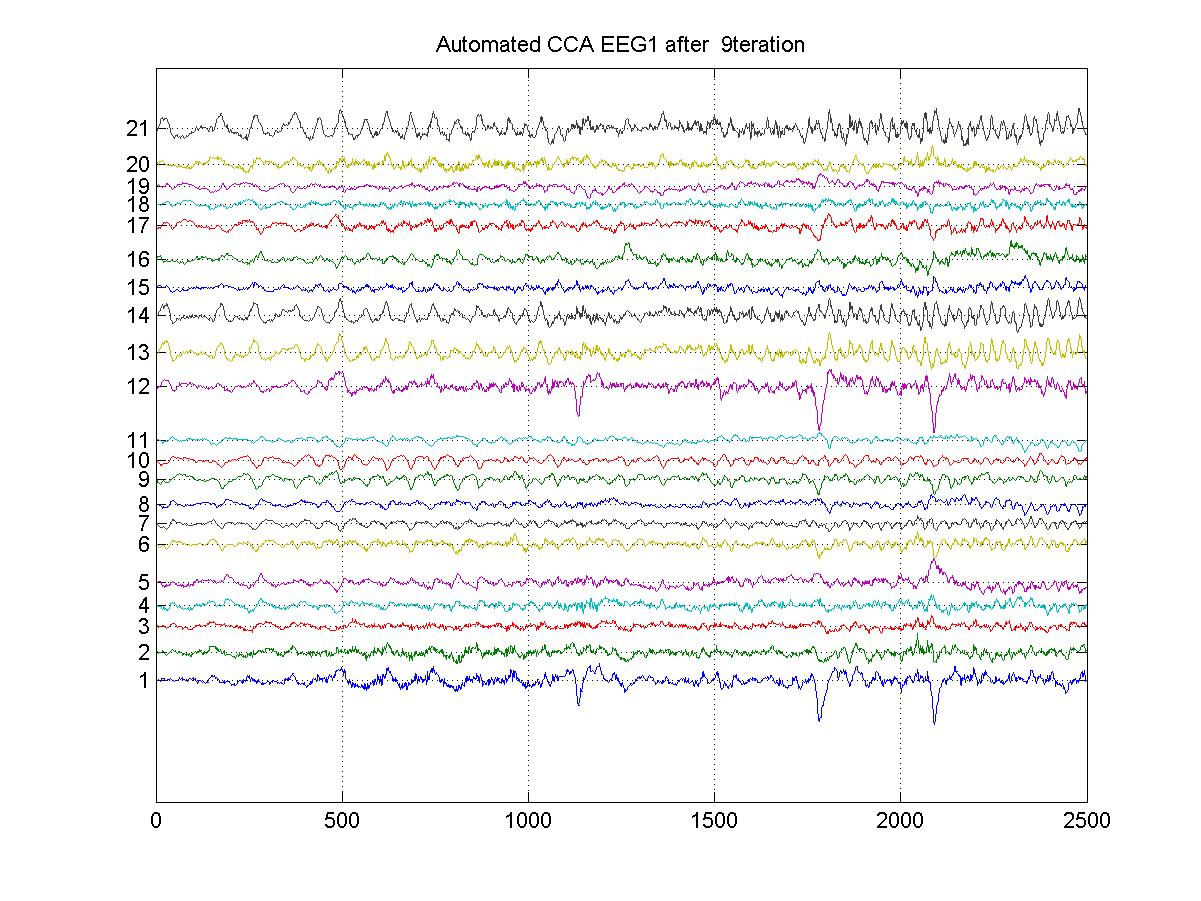
\includegraphics[width=1\textwidth]{35.jpg}
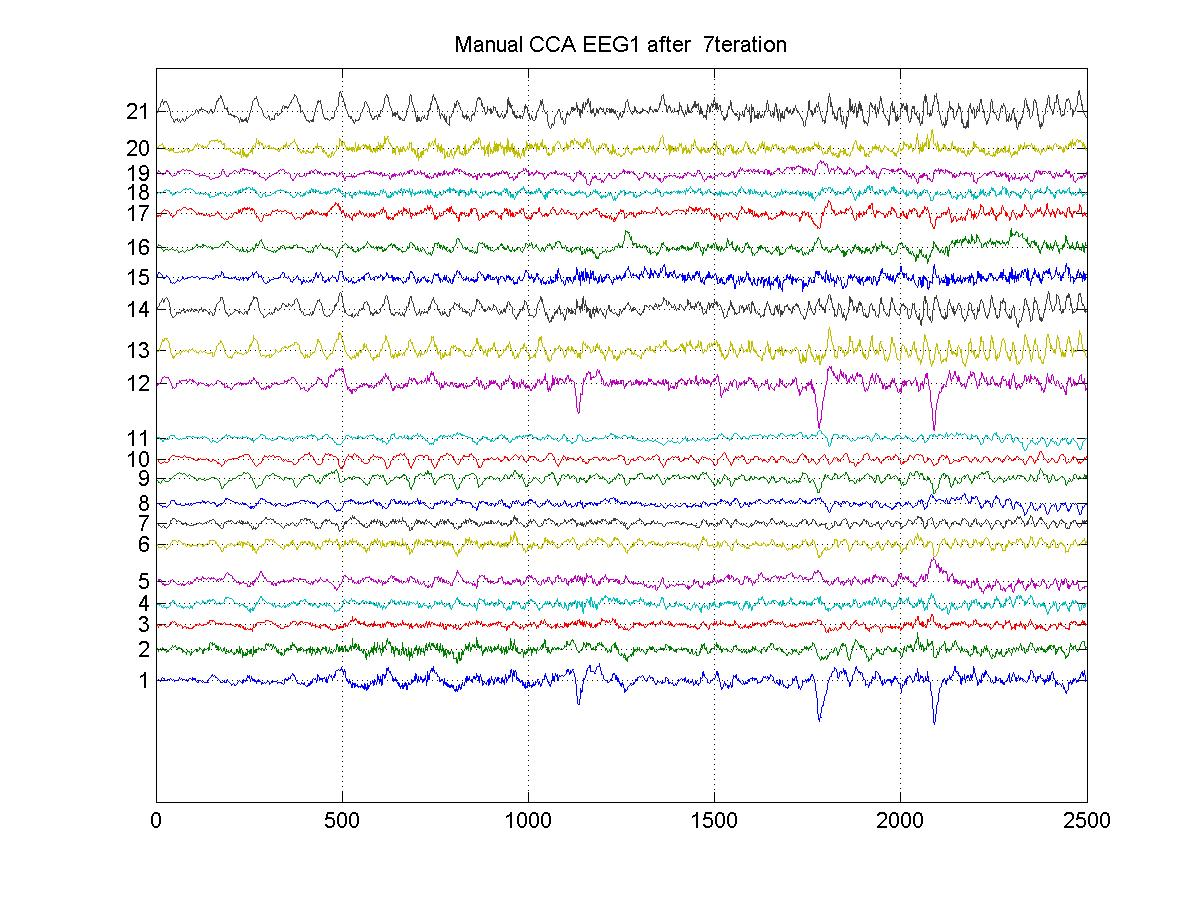
\includegraphics[width=1\textwidth]{721.jpg}
\subcaption{BSS for the dataset EEG1}\label{Nadya6}
\endminipage\hfill
\minipage{0.5\textwidth}%
\centering
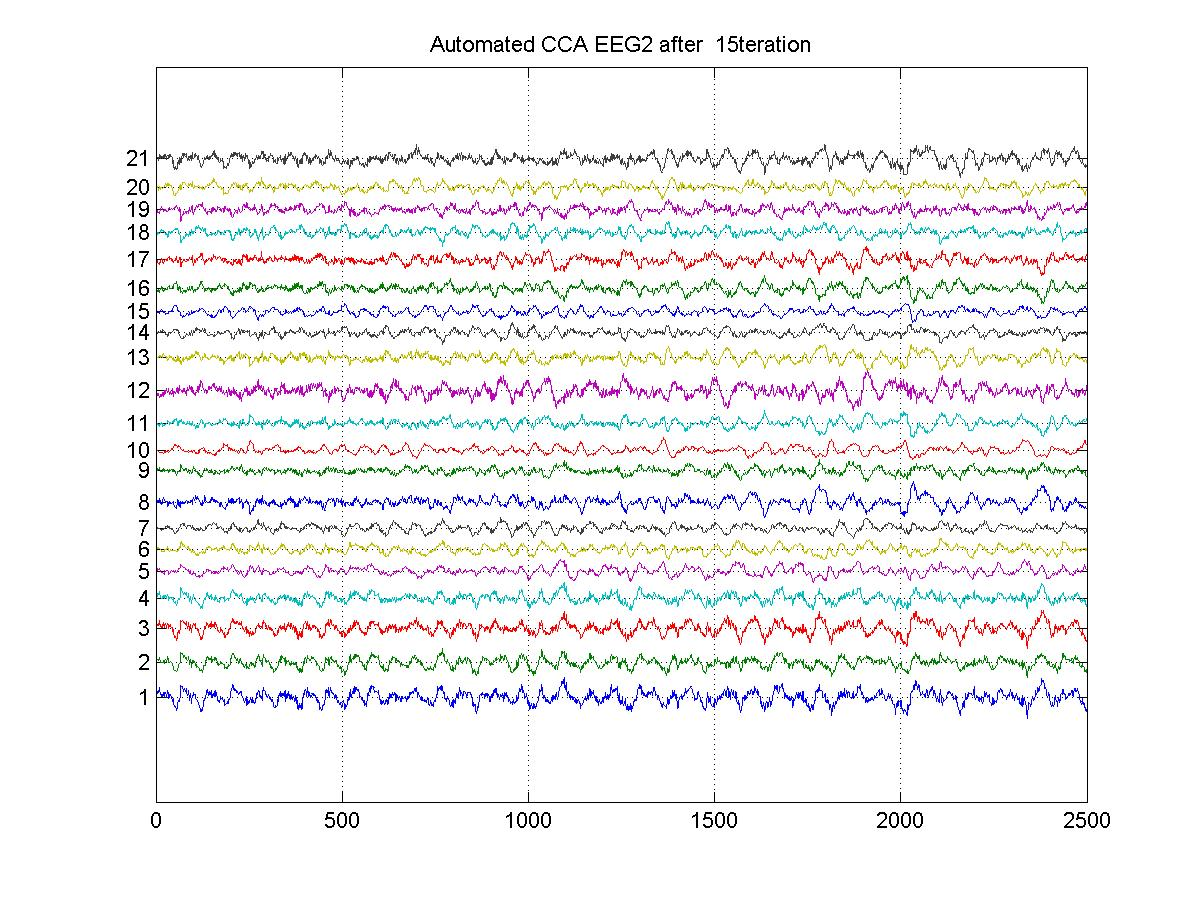
\includegraphics[width=1\textwidth]{81.jpg}
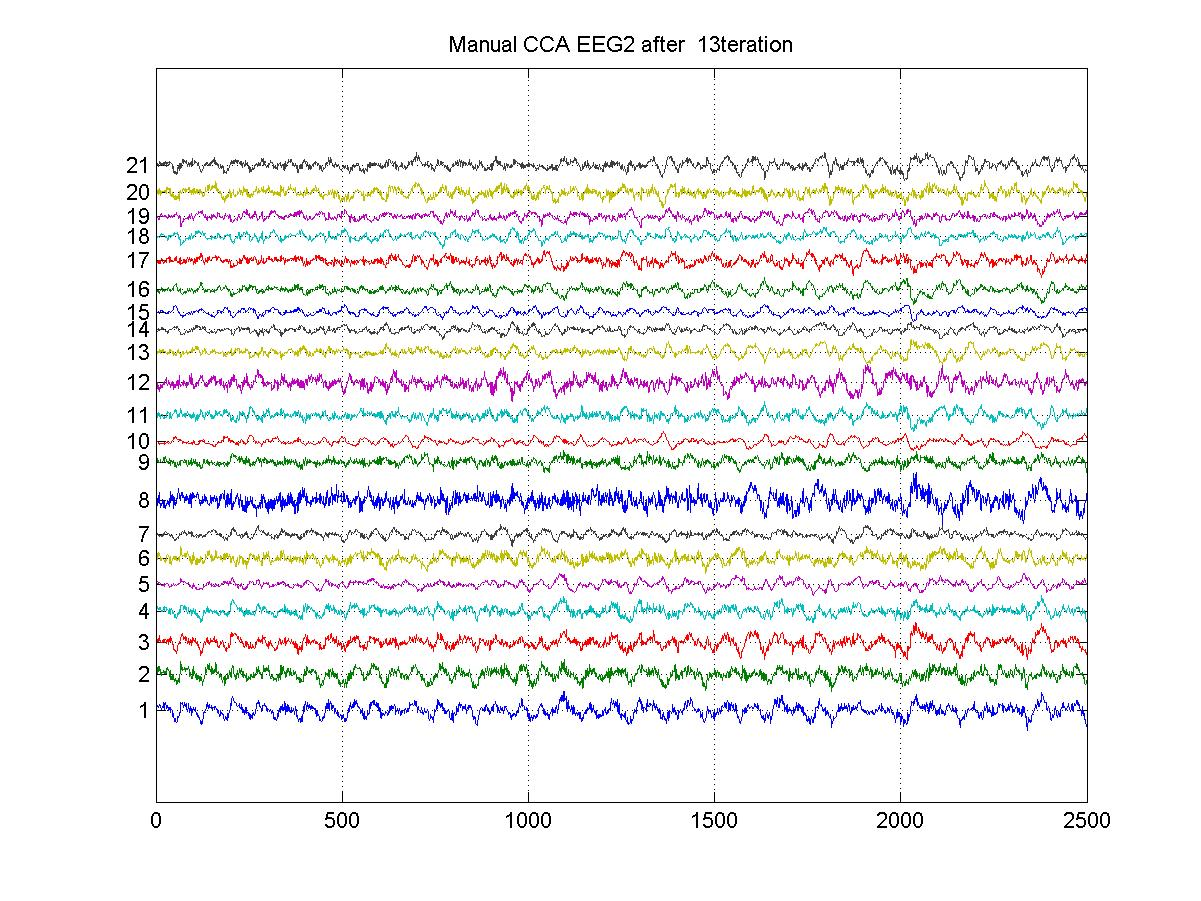
\includegraphics[width=1\textwidth]{761.jpg}
\subcaption{BSS for the dataset EEG2}\label{Nadya7}
\endminipage\hfill
\caption{EEG final results}\label{Perfor}
\end{figure}


\begin{figure}[!htbp]
\minipage{0.5\textwidth}%
\centering
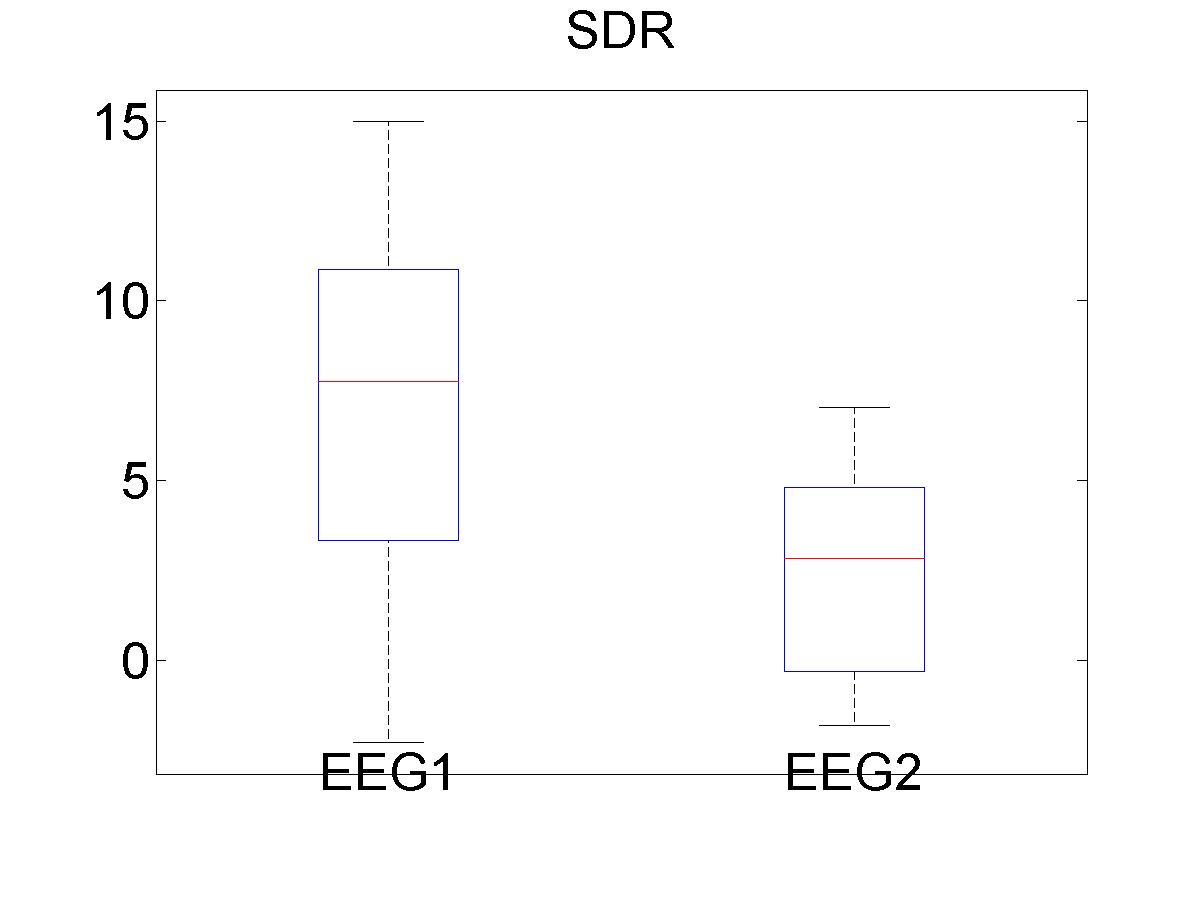
\includegraphics[width=1\textwidth]{82.jpg}
\subcaption{SDR}\label{SAR}
\endminipage\hfill
\minipage{0.5\textwidth}%
\centering
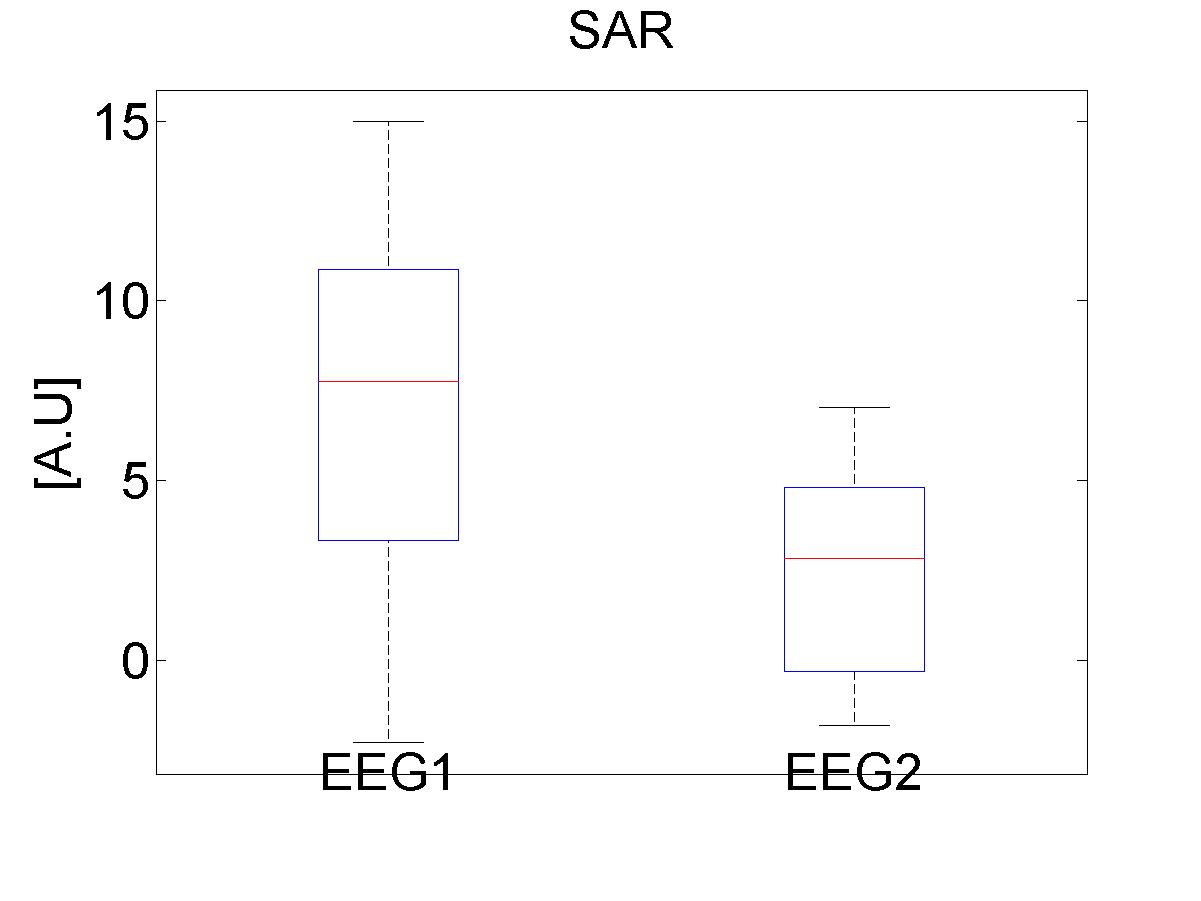
\includegraphics[width=1\textwidth]{83.jpg}
\subcaption{SAR}\label{SDR}
\endminipage\hfill
\caption{BSS performance of the two dataset}\label{Perfor1}
\end{figure}

\begin{figure}[!htbp]
\minipage{0.5\textwidth}%
\centering
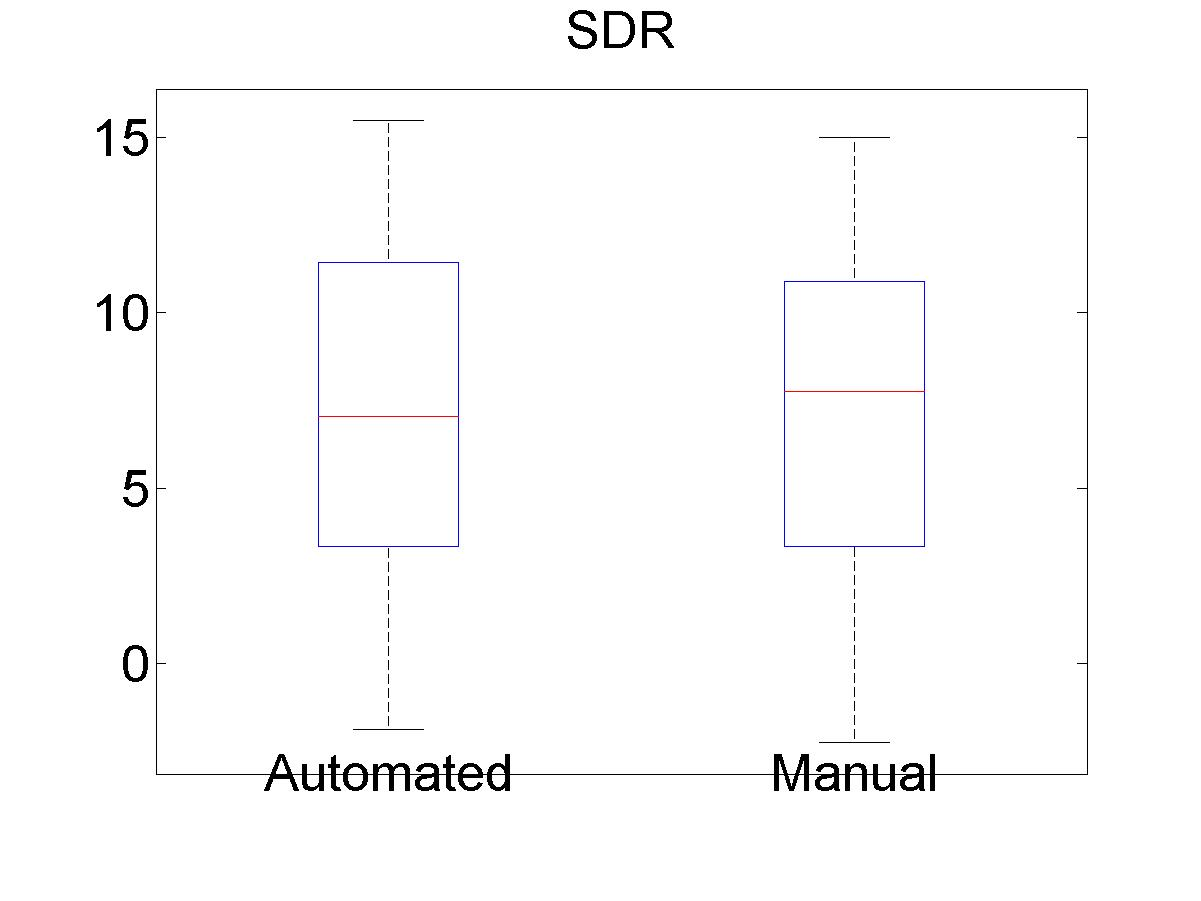
\includegraphics[width=1\textwidth]{84.jpg}
\subcaption{SDR}\label{SAR}
\endminipage\hfill
\minipage{0.5\textwidth}%
\centering
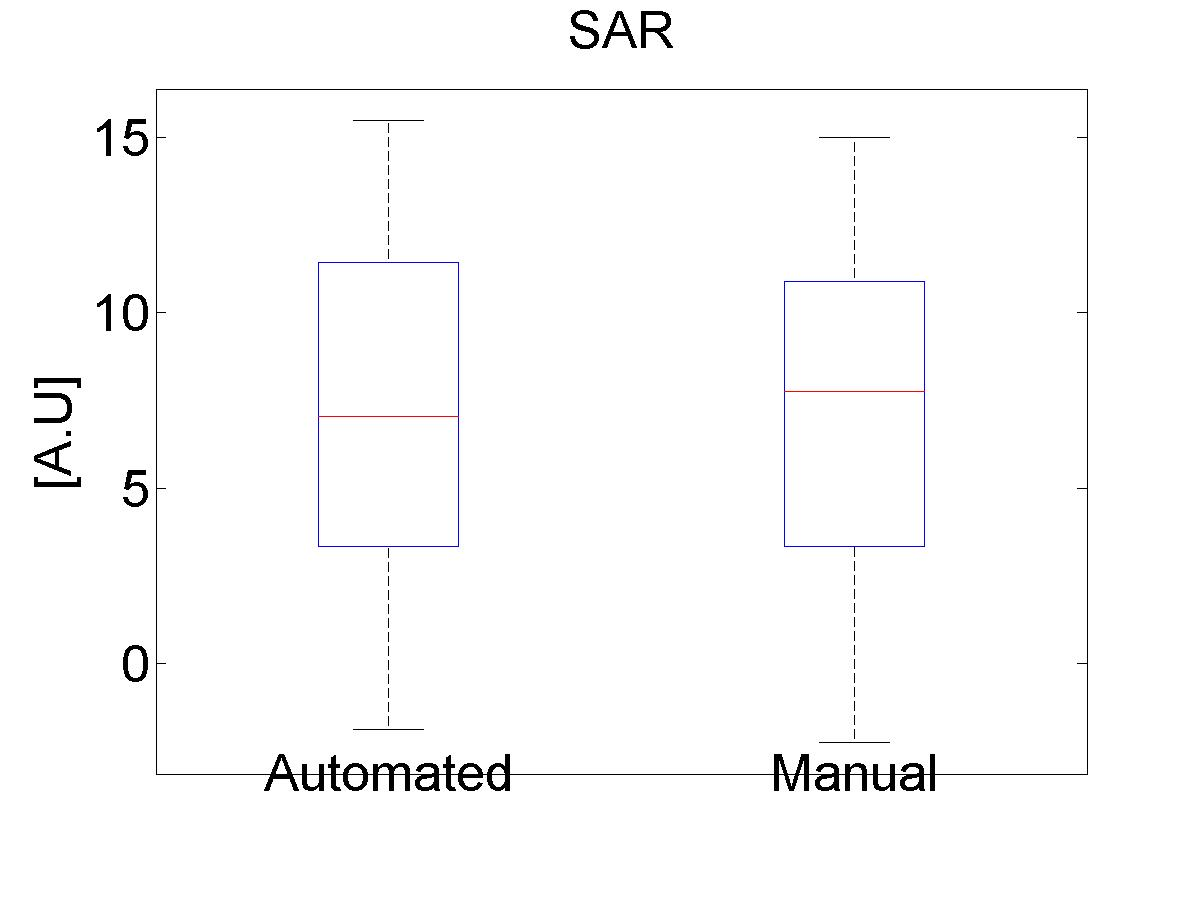
\includegraphics[width=1\textwidth]{85.jpg}
\subcaption{SAR}\label{SDR}
\endminipage\hfill
\caption{BSS performance of automated vs manual CCA}\label{Perfor2}
\end{figure}


\begin{figure}
    \centering
    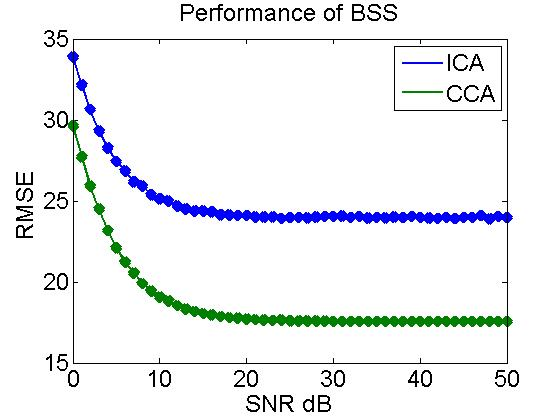
\includegraphics[width=0.48\textwidth]{BSS_Performance.jpg}
    \caption{Caption}
    \label{BSSPerformance}
\end{figure}


Both CCA and ICA perform BSS upon different underlying goals and to compare these methods, root-mean-square-error RMSE has been chosen to evaluate the performance of each. CCA clearly outperforms ICA for different levels of \textbf{wgn} contaminating the channels. This is evidenced in figure \ref{BSSPerformance}. Whereas an arbitrary waveform (mixture of signals) is being utilized for testing the correctness of the ICA in \ref{Test}

\begin{figure}[!htbp]
\minipage{0.5\textwidth}%
\centering
{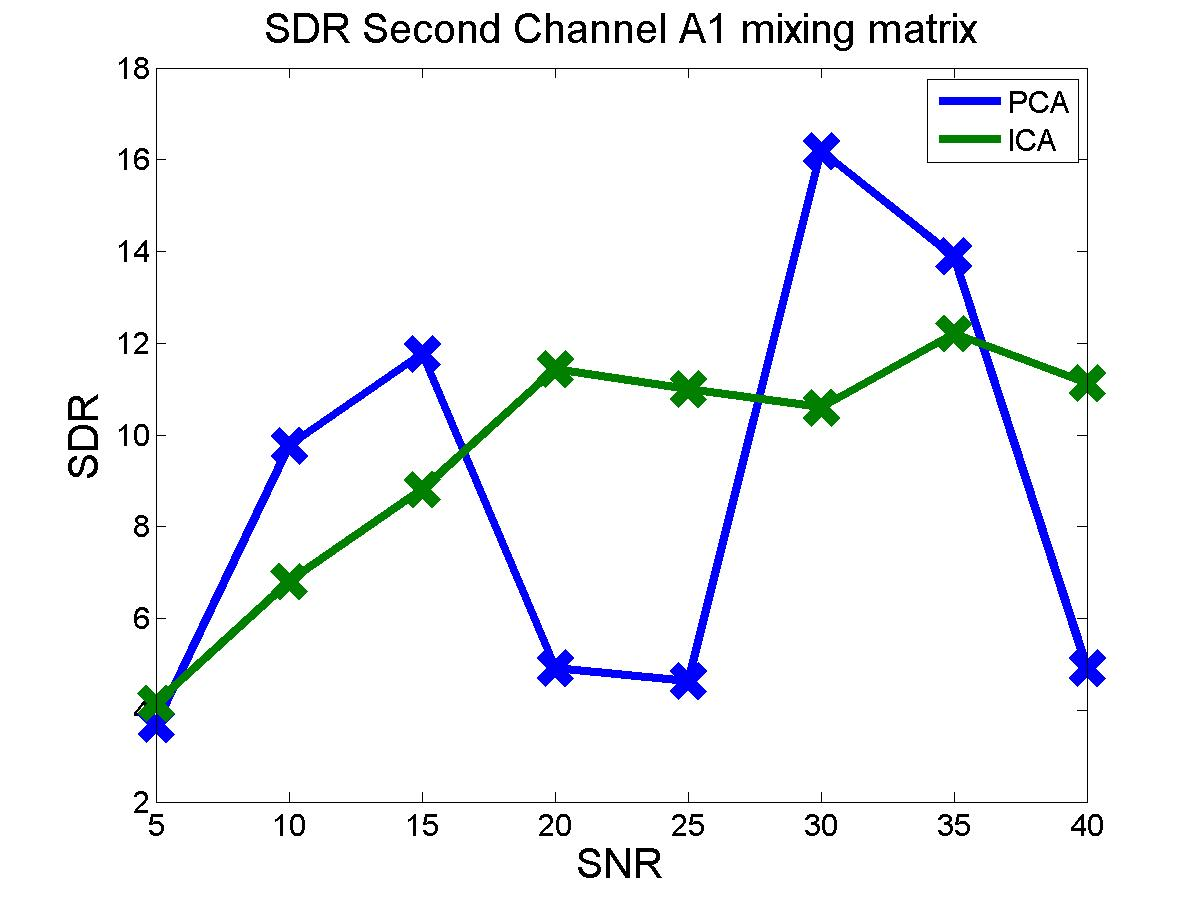
\includegraphics[width=1\textwidth]{2.jpg}};
\subcaption{First data set}\label{Nadya1}
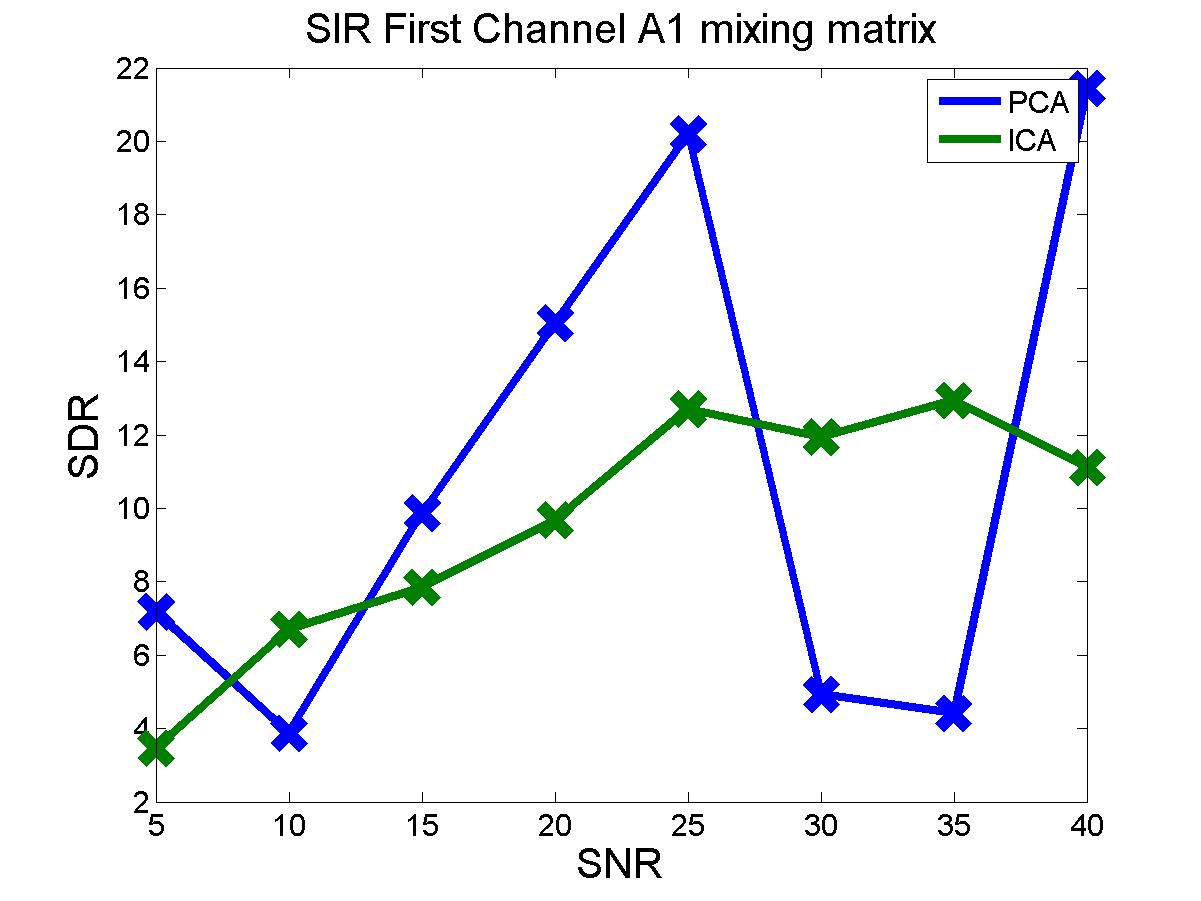
\includegraphics[width=1\textwidth]{5.jpg}
\subcaption{ACS for the dataset EEG1}\label{Nadya5}
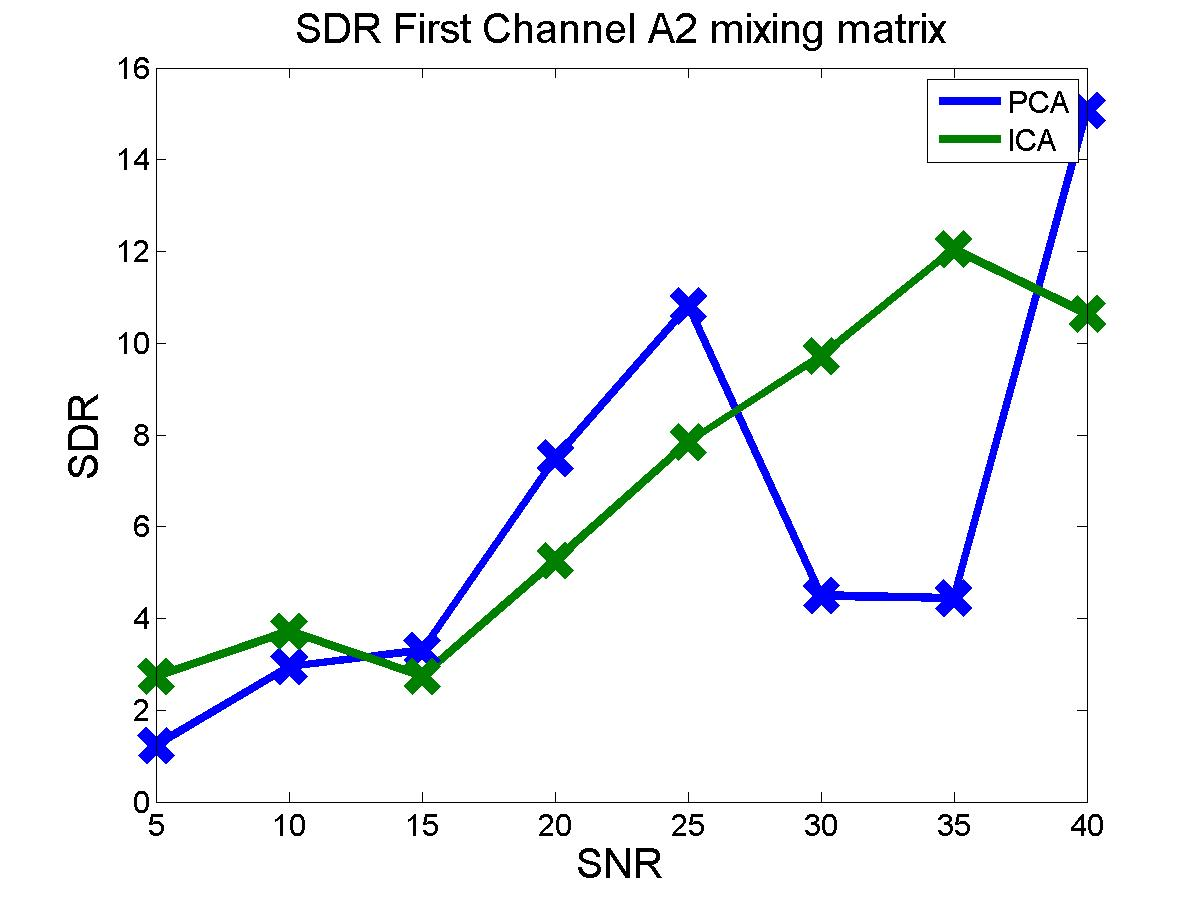
\includegraphics[width=1\textwidth]{3.jpg}
\subcaption{EEG1 CCA channels}\label{Nadya4}
\endminipage\hfill
\minipage{0.5\textwidth}%
\centering
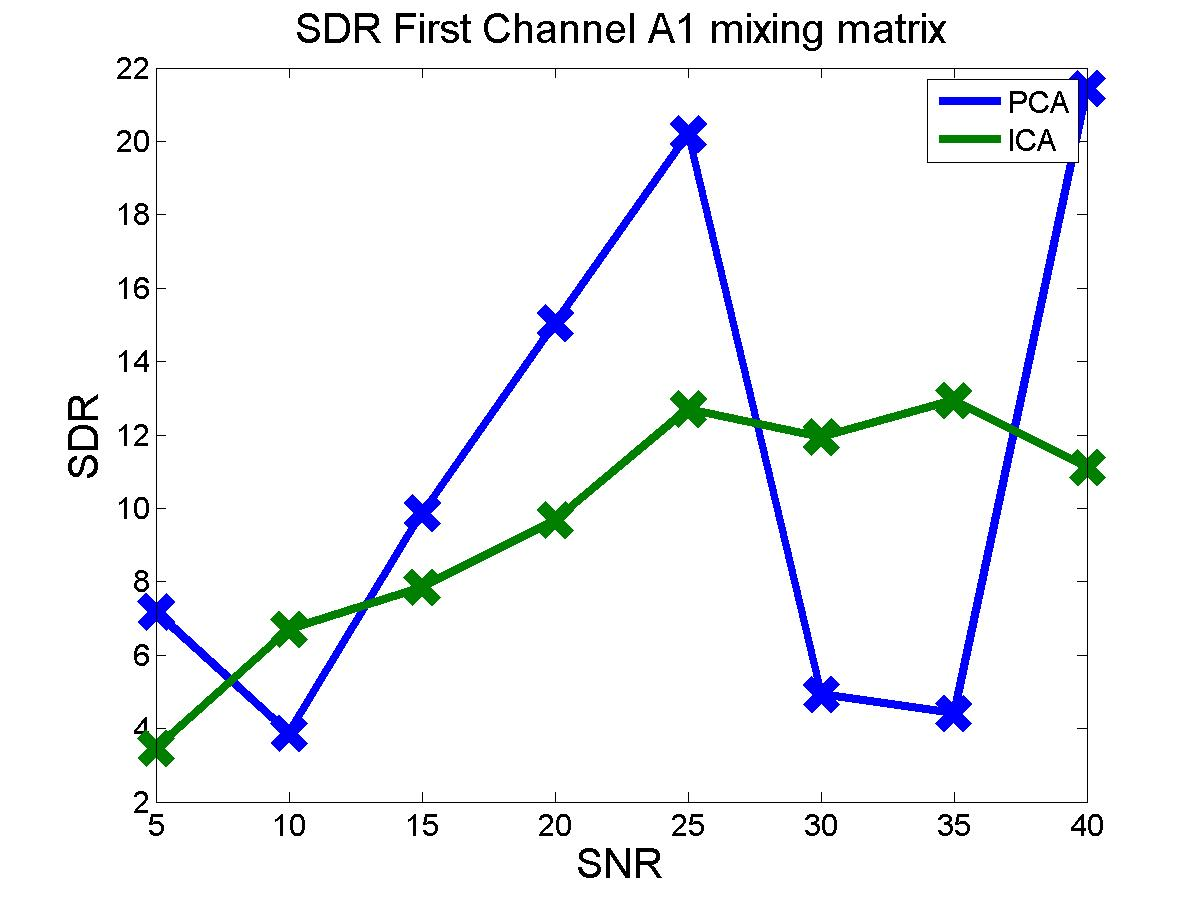
\includegraphics[width=1\textwidth]{1.jpg}
\subcaption{Second data set}\label{Nadya2}
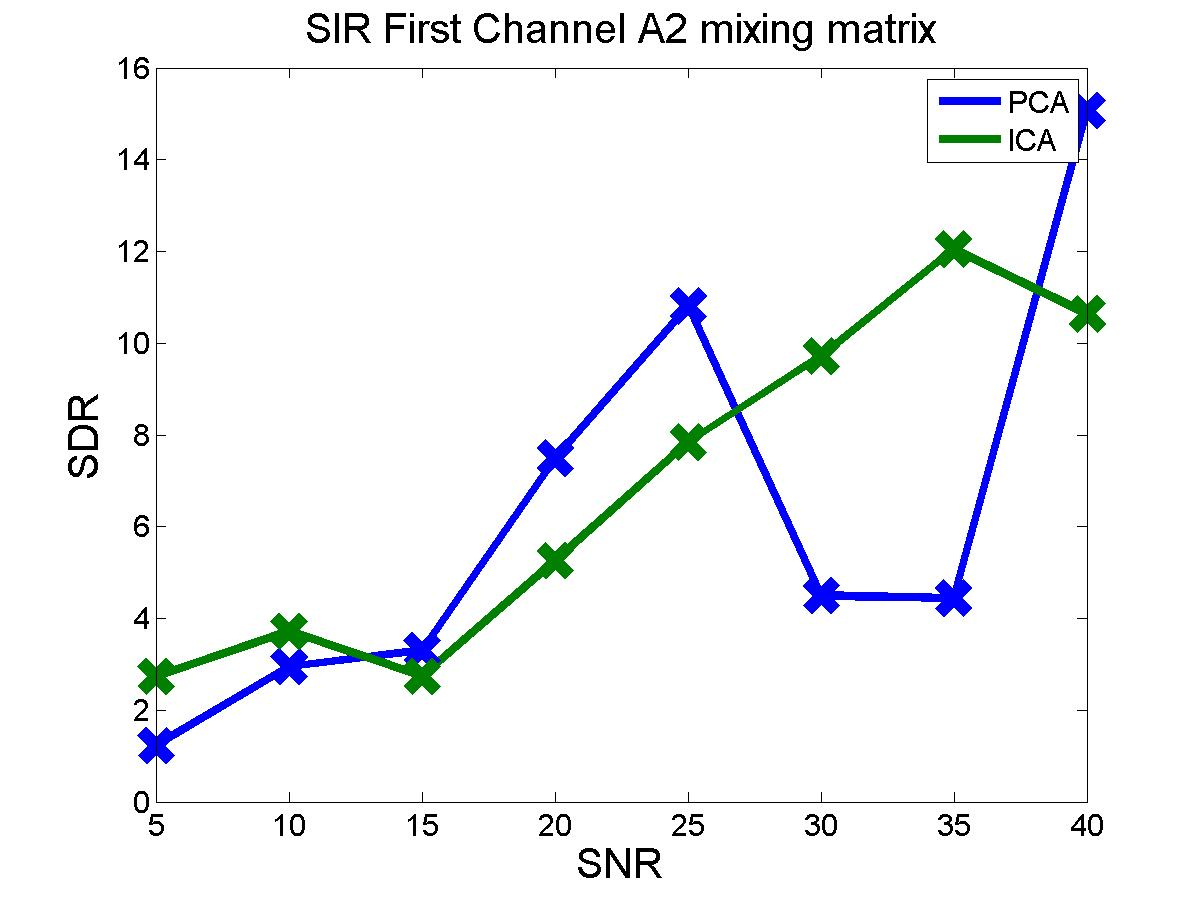
\includegraphics[width=1\textwidth]{7.jpg}
\subcaption{ACS for the dataset EEG2}\label{Nadya8}
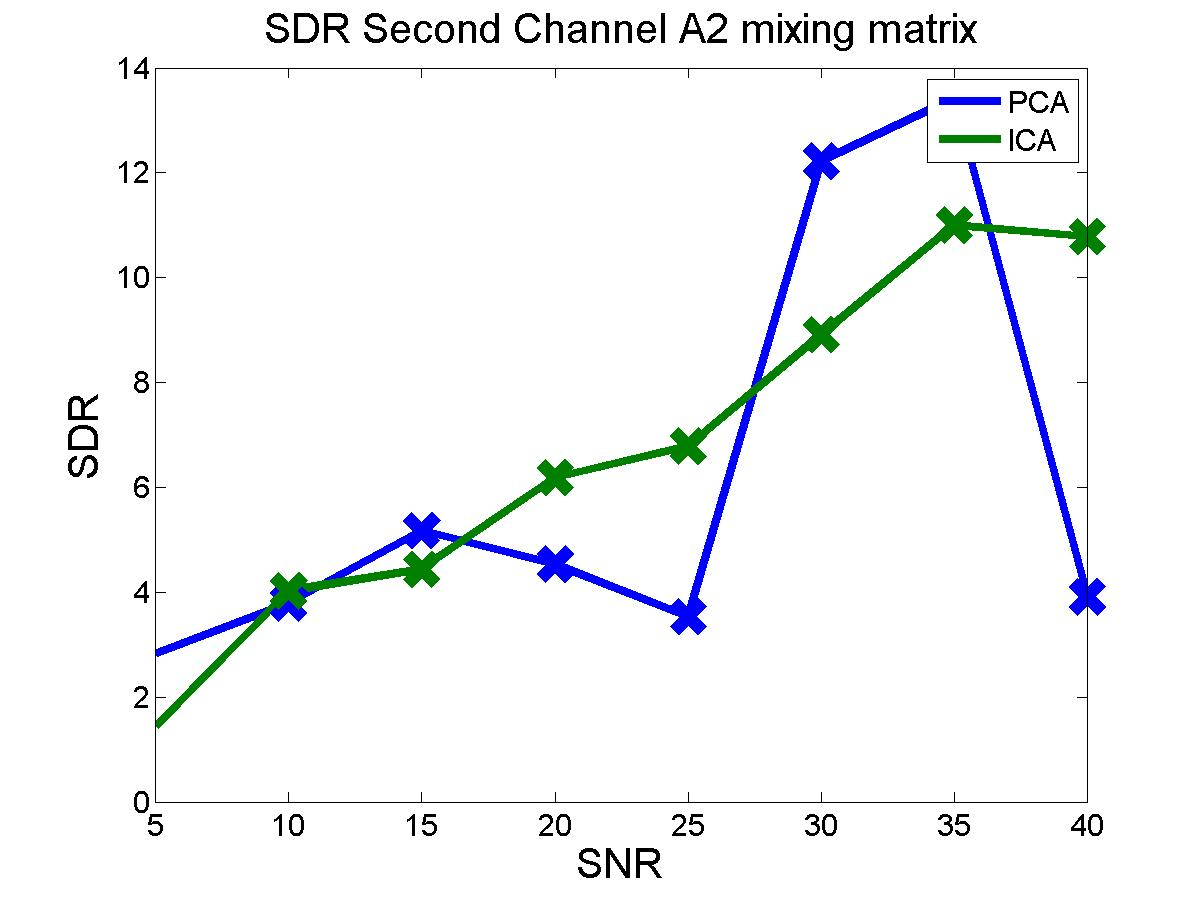
\includegraphics[width=1\textwidth]{4.jpg}
\subcaption{EEG2 CCA channels}\label{Nadya3}
\endminipage\hfill
\caption{EEG dataset}
\end{figure}



\begin{figure}[!htbp]
\minipage{0.5\textwidth}%
\centering
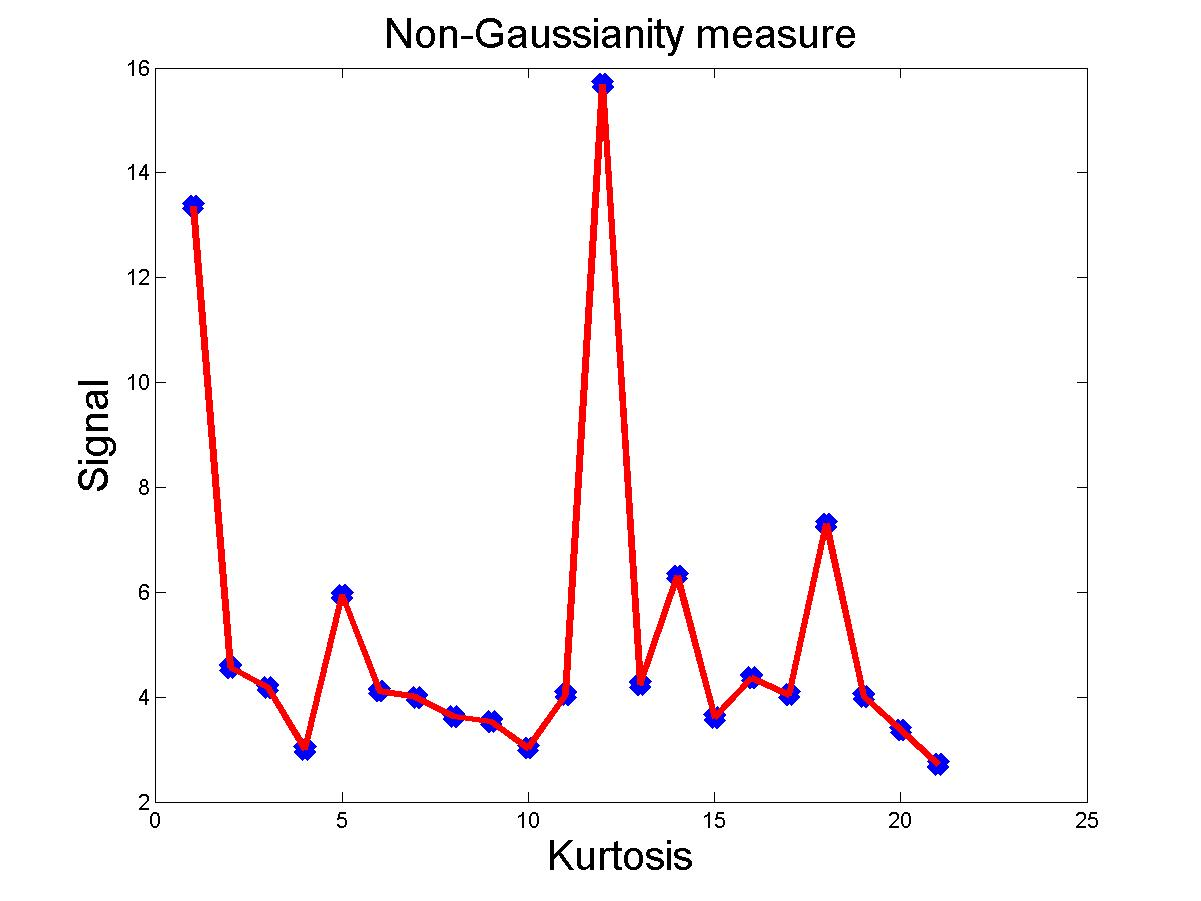
\includegraphics[width=1\textwidth]{500.jpg}
\subcaption{Kurtosis for EEG1}\label{Kurtosis1}
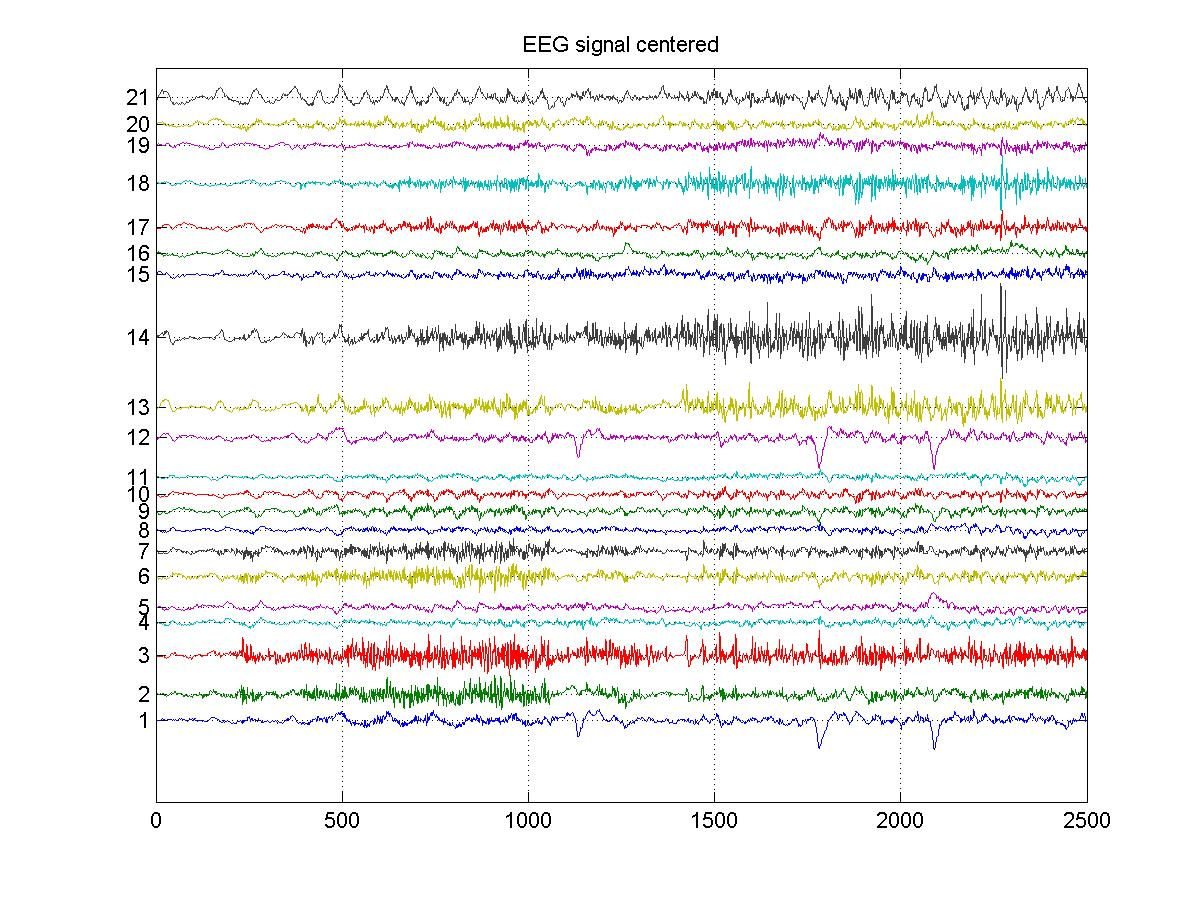
\includegraphics[width=1\textwidth]{503.jpg}
\subcaption{EEG1 centered}\label{center1}
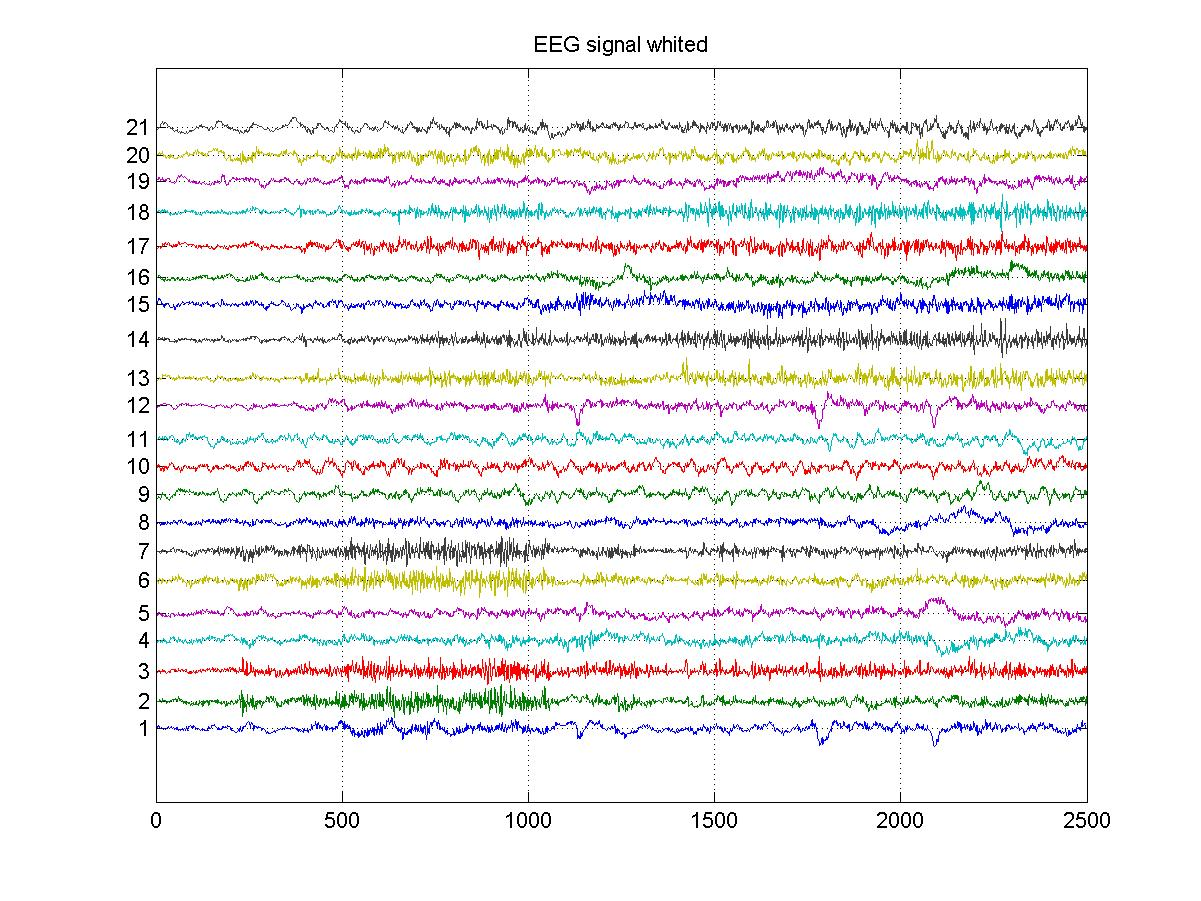
\includegraphics[width=1\textwidth]{504.jpg}
\subcaption{EEG1 whited}\label{whited1}
\endminipage\hfill
\minipage{0.5\textwidth}%
\centering
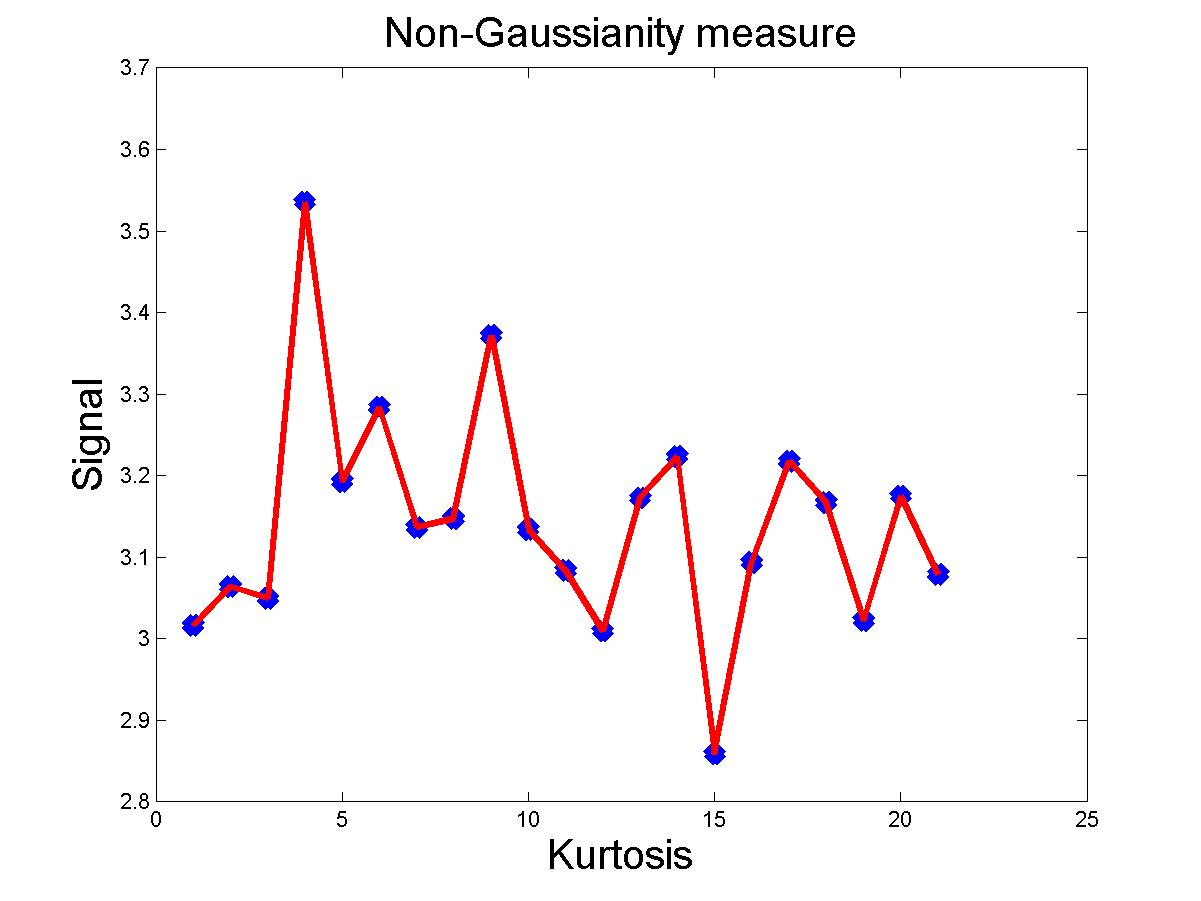
\includegraphics[width=1\textwidth]{501.jpg}
\subcaption{Kurtosis for EEG2}\label{Kurtosis2}
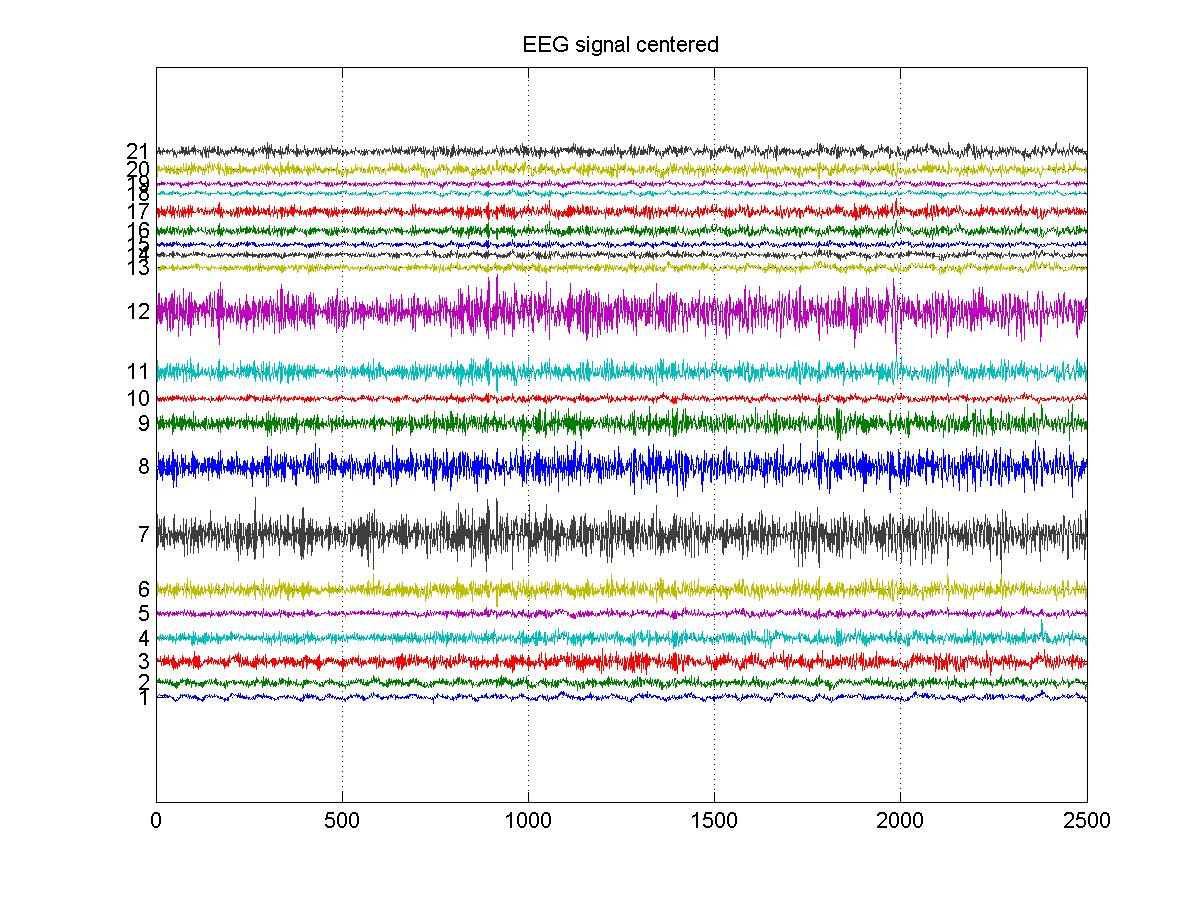
\includegraphics[width=1\textwidth]{509.jpg}
\subcaption{EEG2 centered}\label{center2}
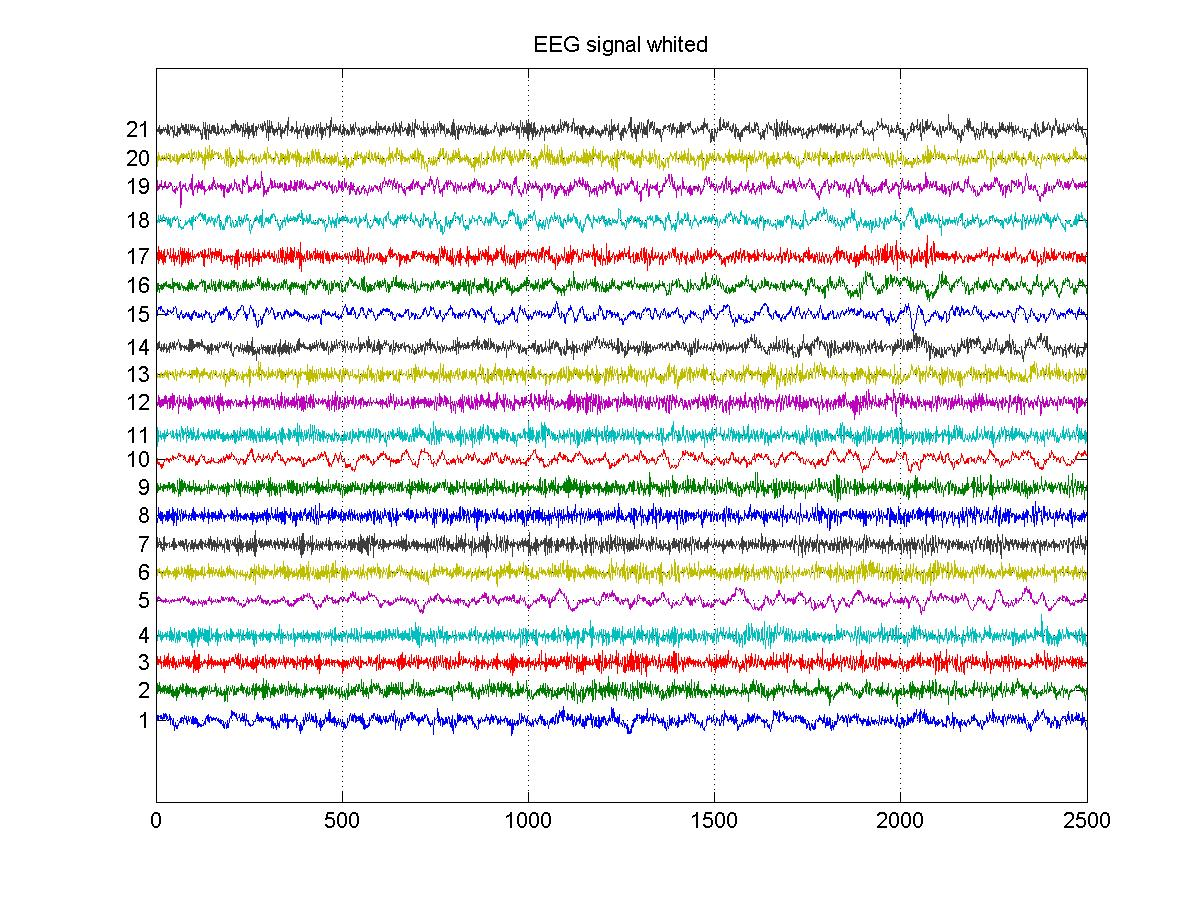
\includegraphics[width=1\textwidth]{510.jpg}
\subcaption{EEG2 whited}\label{whited2}
\endminipage\hfill
\caption{ICA preprocessing data}
\end{figure}



\begin{figure}[!htbp]
\minipage{0.5\textwidth}%
\centering
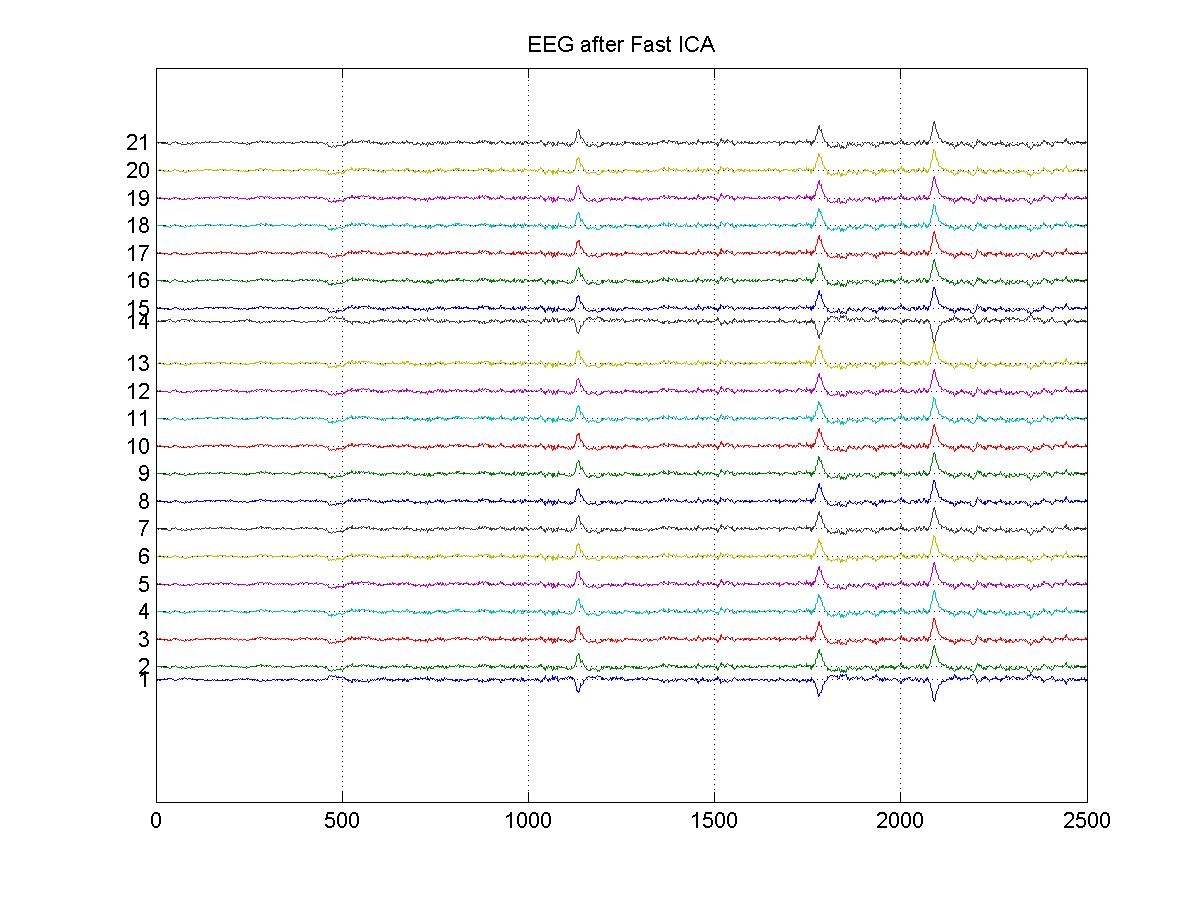
\includegraphics[width=1\textwidth]{505.jpg}
\subcaption{BSS of the EEG1}\label{BSS1}
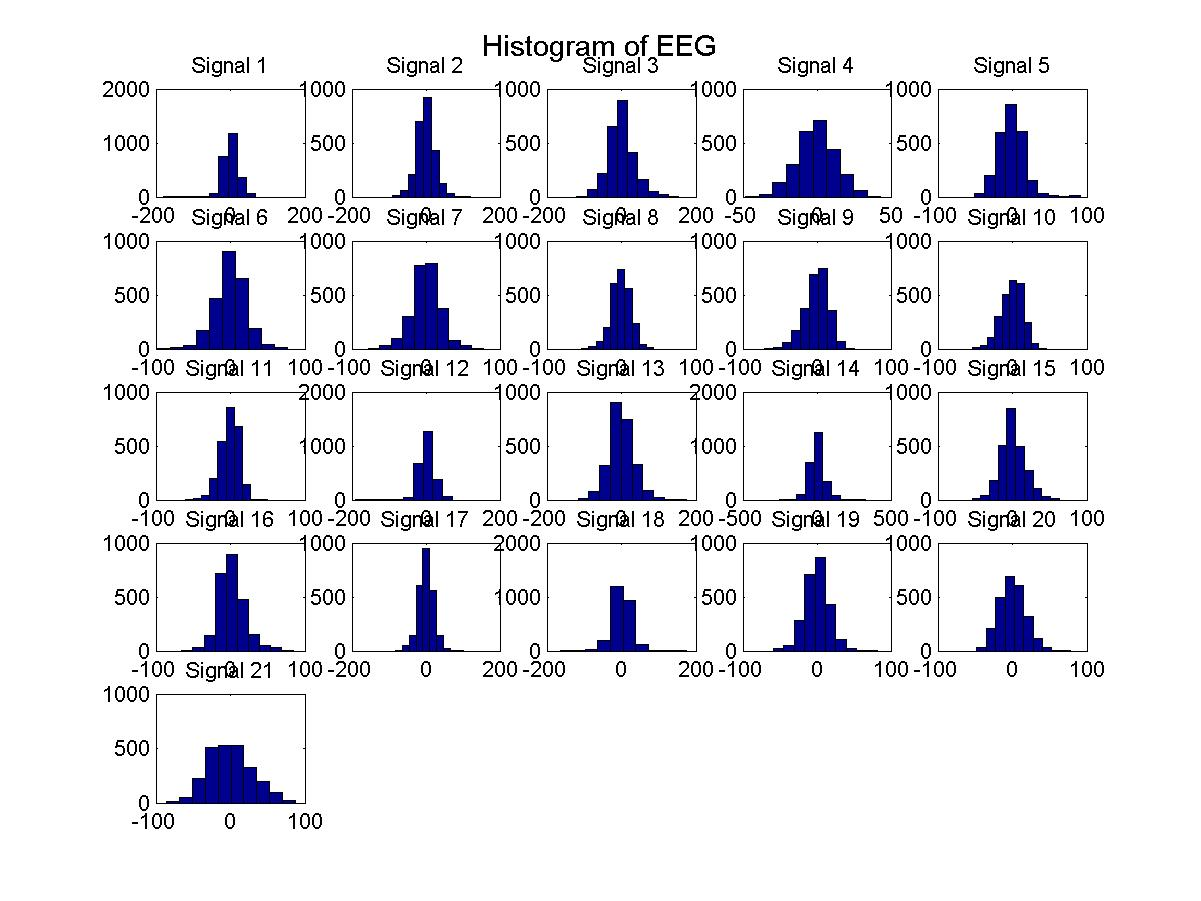
\includegraphics[width=1\textwidth]{506.jpg}
\subcaption{EEG1 hist before ICA}\label{HIST1}
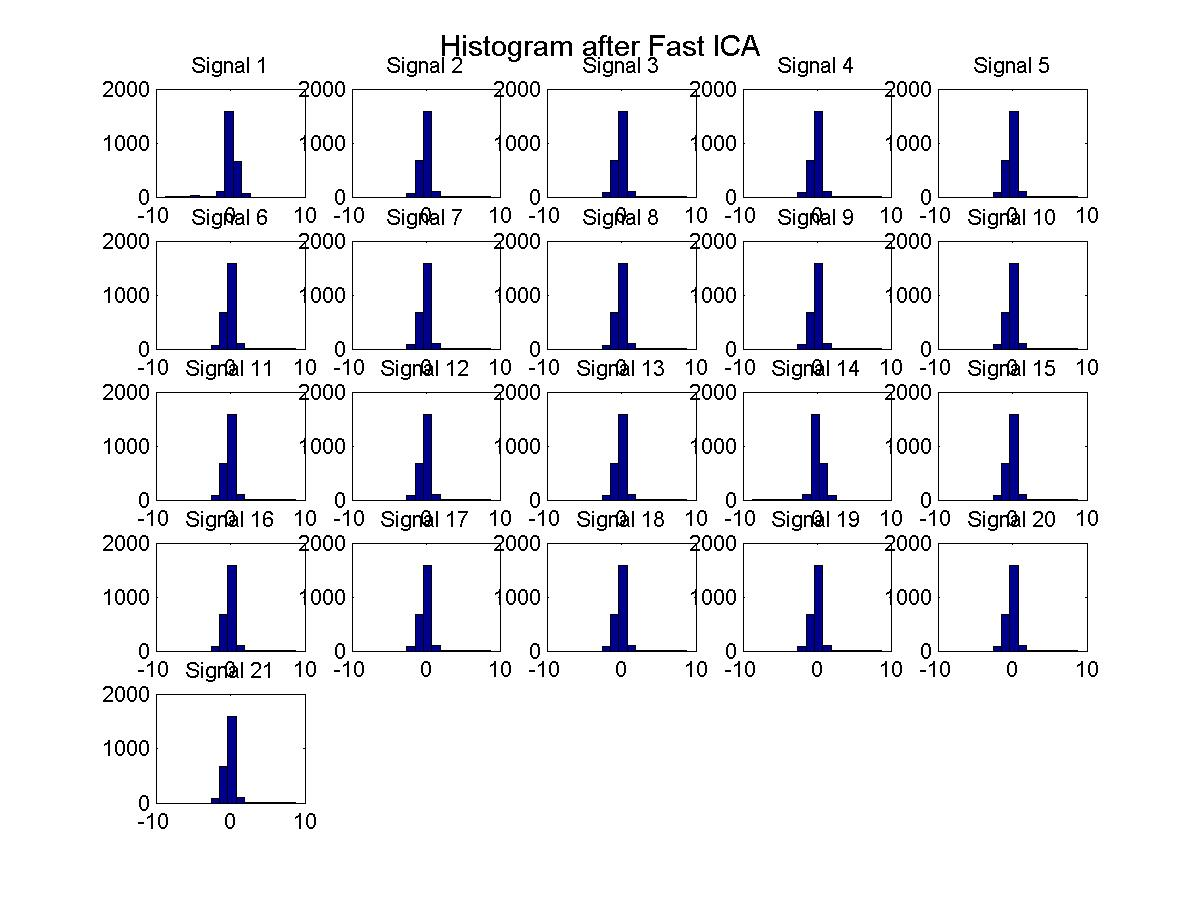
\includegraphics[width=1\textwidth]{507.jpg}
\subcaption{EEG1 hist before ICA}\label{HIST3}
\endminipage\hfill
\minipage{0.5\textwidth}%
\centering
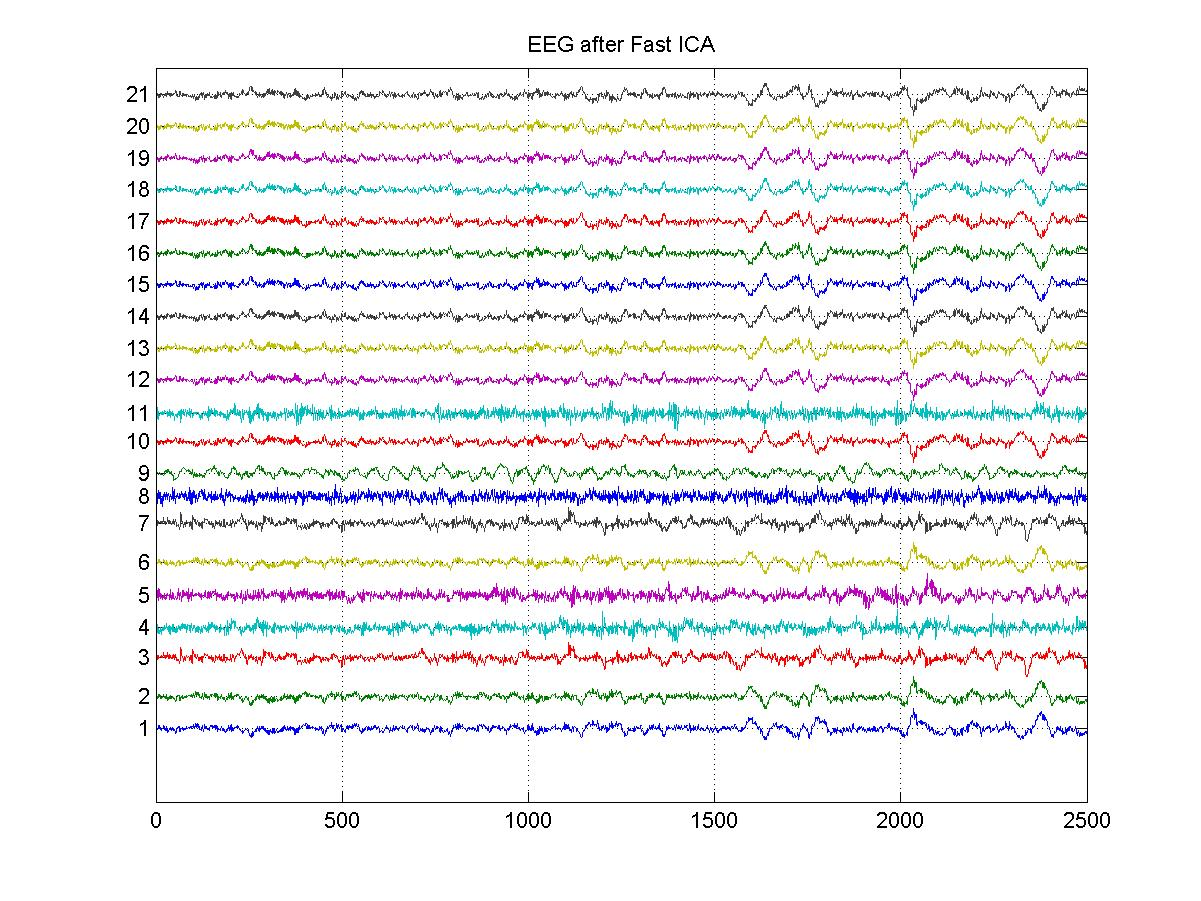
\includegraphics[width=1\textwidth]{511.jpg}
\subcaption{BSS of the EEG2}\label{BSS2}
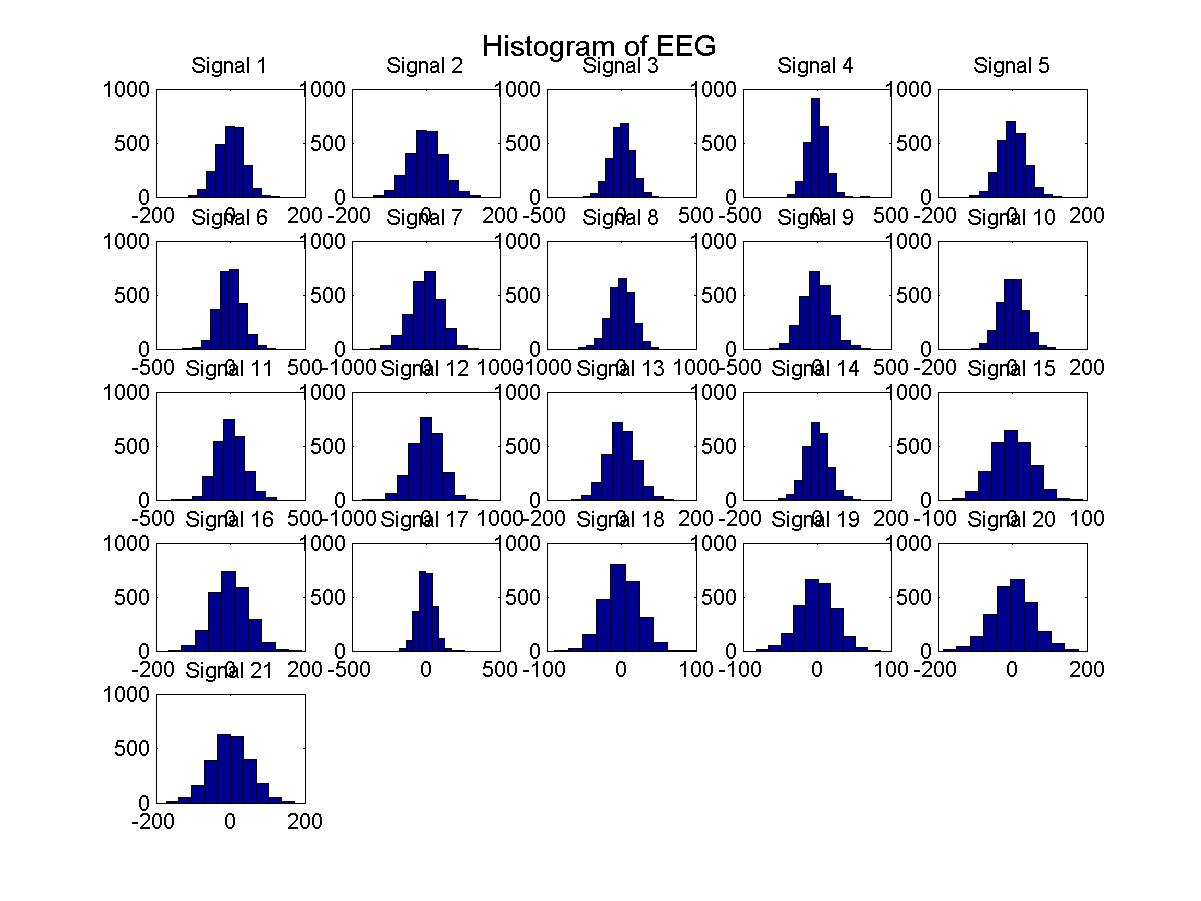
\includegraphics[width=1\textwidth]{512.jpg}
\subcaption{EEG1 hist before ICA}\label{HIST2}
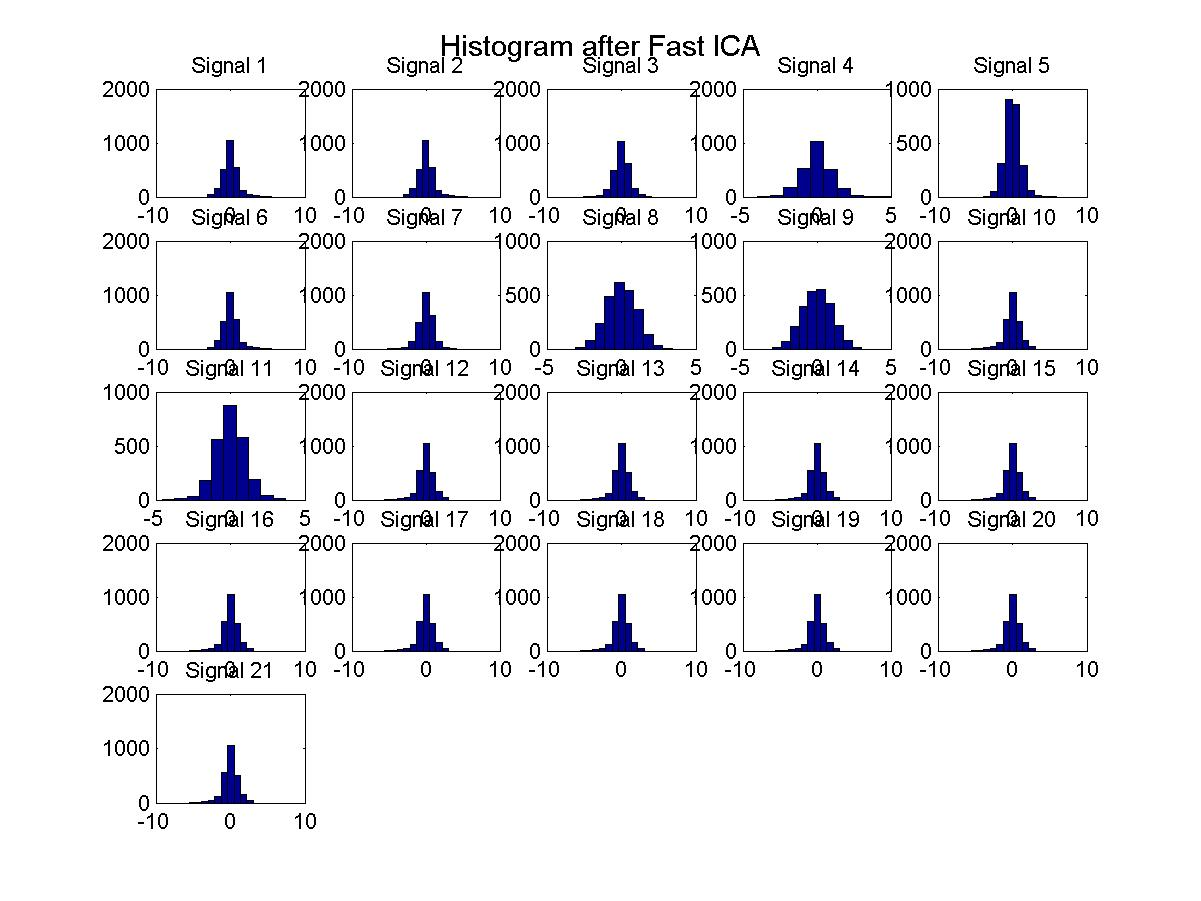
\includegraphics[width=1\textwidth]{513.jpg}
\subcaption{EEG1 hist before ICA}\label{HIST4}
\endminipage\hfill
\caption{EEG dataset}
\end{figure}



\newpage
\subsection{Differences between CCA and ICA}


\begin{itemize}

\item CCA performs the BSS much better than ICA which is testified with the RMSE performance plot for different noise levels.

\item CCA is straight forward implemented, meaning that there is no need to iteratively solve or optimize any parameter. Whereas ICA employees an iterative method for the separation of sources by maximizing their non-Gaussianity \cite{15}. Consequently, it requires much higher time complexity compared to CCA. CCA employs matrix decomposition at a single iteration.  

\item Via ICA-BSS there is no guarantee for the same output for identical data contrary to the CCA, which can reproduce the data for the same input. This is mainly due to the fact that ICA outcome depends on the number of iterations and the input parameters\cite{16}. It means that outcome arises at one iteration. The outcome of the ICA strictly depends on the data set values meaning that optimization process and the number of iteration has a certain variability. 

\item Even though both of the methods try to separate the sources, the consideration is different in both cases. CCA tries to make the sources as less uncorrelated as possible and maximize the autocorrelation of channels whereas ICA tries to make the sources as less independent as possible. Statistically speaking, independence is far stronger than uncorrelatedness. meaning that independence implies the uncorrelatedness whereas the other way around does not stand. In other words, uncorrelatedness is just an instance of independence\cite{15}. 

\item Differently from the CCA case, ICA assumes the input data set to be full non-Gaussian\cite{15}. Even though natural events rarely contradict with the central limit theory CLT, in some biomedical signal in particular non-Gaussianity is still no prevalent. CCA does not depend on this assumption, thereby it performs the separation at any type signals which are non correlated.

\item ICA in addition requires pre-processing  of the data, including here centering and whitening of the data\cite{15}. CCA does the separation straight from the raw data without the need of any pre-processing. Despite the pre-processing incorporated into the ICA, yet the method tends to be reluctant to the robustness due to the assumption of neg-entropy and kurtosis estimation for the non-Gaussianity \cite{17}. 

\item Auto-correlation is a well defined method, thereby the correlation coefficients between the sources to be proceeded are defined very accurately in a very robust manner. The outcome is afterwards linearly processed with the aim of a separation of the sources. Whereas in the ICA, independence remains solid in multiple prospective.  

\end{itemize}
\section{PCA vs ICA}

The general aim of the BSS of a data matrix \textbf{X} is to decompose this matrix into mixing matrix \textbf{A} scaling matrix \textbf{D}$=diag(\lambda_{1},\lambda_{2},\lambda_{3},\cdots,\lambda_{R})$ and matrix of the unknown source \textbf{B} \cite{3}. The general notation is as in the equation \ref{eq1}. The matrix \textbf{e} is noise which is presented in any underlying model.

\begin{equation}\label{eq1}
    X=ADB^{T}+e
\end{equation}

Principal component analysis PCA and independent component analysis ICA are the two main approaches being explored in here. Both this method are linear and nonparametric method which try to separate separate the the linearly mixed source  \cite{1},\cite{2}. 

PCA gets the mixed channels and try to center each channel. Upon this centered data the covariance matrix is computed. Since the covariance matrix is not diagonal the covariance coefficients testify a linear relation of each channels. A linear transformation of the data is required where its respective covariance matrix is now fully diagonal (i.e. the new features are uncorrelated). This is performed either via eigenvalue decomposition (EVD) or singular value decomposition (SVD) \cite{1} where the final matrix will be the mixing matrix A the scaling diagonal matrix B and the principal component which are orthogonal. 

The values in the diagonal matrix \textbf{D} are the variance of each channel sorted into descending order. High values of $\lambda$ reveal high dynamics consequently high amount of information is unclosed into that respective subspaces. The last value of the diagonal is the variance of the channel with noise therefore the corresponding subspace is the most unrelated component. 

In the orthogonal matrix D are concatenated the principal component also known as the dimension of the measurements sorted by their importance. From the BSS prospective these component are the original source to be linearly mixed with the mixing matrix \textbf{A}. 

ICA on the other hand, tries to separate the sources by making them independently (i.e. the covariance matrix is diagonal). Independence is a stronger condition than uncorrelated. Signals are uncorrelated if their covariance is zero:

\begin{equation}\label{equati1}
E(y_{1}y_{2})-E(y_{1})E(y_{2})=0
\end{equation}

Signals are independent if their joined probability is equal the production of the respective probability:

\begin{equation}\label{equati2}
p(y_{1}y_{2})=p(y_{1})p(y_{2})
\end{equation}

Independence by default includes the uncorrelated condition whereas the other way around is not true. ICA does the decomposition yet consistently to the equation \ref{eq1} with minor differences.

The general formulation is $X=MY+e$ where M is the mixing matrix whereas Y are the original (independent) sources to be estimated and \textbf{e} is the noise superimposed over the underlying model. 
The main mathematical differences between ICA and PCA are listed below:

\begin{itemize}
    \item ICA works on non-Gaussian data whereas PCA on Gaussian data
    \item ICA works on high order statistics whereas PCA on mean and variance.
    \item ICA doesn't do the decomposition into orthogonal sources whereas PCA produces orthogonal estimated sources (ES).
    \item ICA doesn't produces the scaling matrix from the decomposition. ICA doesn't ensure the correct scale of the ES. 
    \item ICA does not ensure the correct ordering of the estimated sources whereas PCA does sort the ES.
    \item ICA does not ensure the phase of the ES whereas PCA does ensure the ordering\cite{4}. 
\end{itemize}

Hereby a study comparative study is performed on two channels drawn from normal distribution. These channels are mixed linearly using two different mixing matrices A1 and A2 in \ref{A2}. The BSS is performed over different level of noise and it has been evaluated via signal to distortion ration SDR, signal to interference ration SIR and signal to artifact ration SAR \cite{6}. 

PCA performance is quite insensitive to noise whereas ICA testifies an enhancement of the performance as the SNR values increases figure \ref{fig1} and \ref{fig2}. This is due to the fact that noise is always concatenated in large scale into the last subspace.  

Additionally PCA performs a much better BSS compare to ICA according to the box plots in figure \ref{fig3}. This occurs due to Gaussianity distribution of the channel data which are not suitable for ICA. 

The norm of the matrix A1 and A2 are respectively 3 and 21 that means a sufficient distance from the singularity. Consequently their inverse matrix does exist. In case the mixing matrix has a conditioning near to singularity its  inverse matrix would not exist therefore the BSS would not be possible. 

\begin{figure}[!htbp]
\foreach \i in {1,...,6} {
    \begin{subfigure}[p]{0.5\textwidth}
        \includegraphics[width=0.9\linewidth]{\i}
    \end{subfigure}\quad
}
\caption{BSS evalution of PCA and ICA}\label{fig1}
\end{figure}

\begin{figure}[!htbp]
\foreach \i in {7,...,12} {%
    \begin{subfigure}[p]{0.5\textwidth}
        \includegraphics[width=0.9\linewidth]{\i}
    \end{subfigure}\quad
}
\caption{BSS evalution of PCA and ICA}\label{fig2}
\end{figure}


\begin{figure}[!htbp]
\foreach \i in {15,...,17} {%
    \begin{subfigure}[p]{0.33\textwidth}
        \includegraphics[width=0.9\linewidth]{\i}
    \end{subfigure}\quad
}
\caption{PCA vs ICA}\label{fig3}
\end{figure}


The correctness of the Fast-ICA has been tested with arbitrary waveform and the result could be found in \ref{A1}.

\section{FECG analysis}
FECG is the fetal ECG superimposed over the maternal ECG. ECG measurement is a cocktail party where on source is measured over different electrodes.

Application of the ICA on the FECG data tends to decrease the interference coming from other sources at the region where the electrodes of the interest is placed. However in this "cocktail" effect the outcome is not with benefits in all the cases. Hereby in figure \ref{FECG1} and \ref{FECG1} the signals before and after applying BSS-ICA. The original signal tends to contain a lot of interference where fetal signal with small amplitude is also incorporated into the underlying signal. This peaks could potentially disappear after the ICA since their correlation with noise is much higher compare to the correlation with the real high amplitude signal. Consequently after ICA these peaks mainly disappear.  Nevertheless these weak fetal signal could potentially be important information for the analysis and risk assessment of the fetal. 

BSS over this dataset is quite efficient where a clear QRS signal is feasible together with the P and T waves which are visually disclosed from the figure \ref{FECG1}. The artefat and the crosstalk that presented in the original signal are suppressed and the quality of the final signal is sufficiently good.

Even though ICA is a very powerful tool in processing ECG signals it is still not a suitable framework for fetal ECG processing. Further processing of the FECG signal could be of great importance using wavelet and filtering in order to extract more hidden information. 

\begin{figure}[!htbp]
\minipage{0.5\textwidth}%
\centering
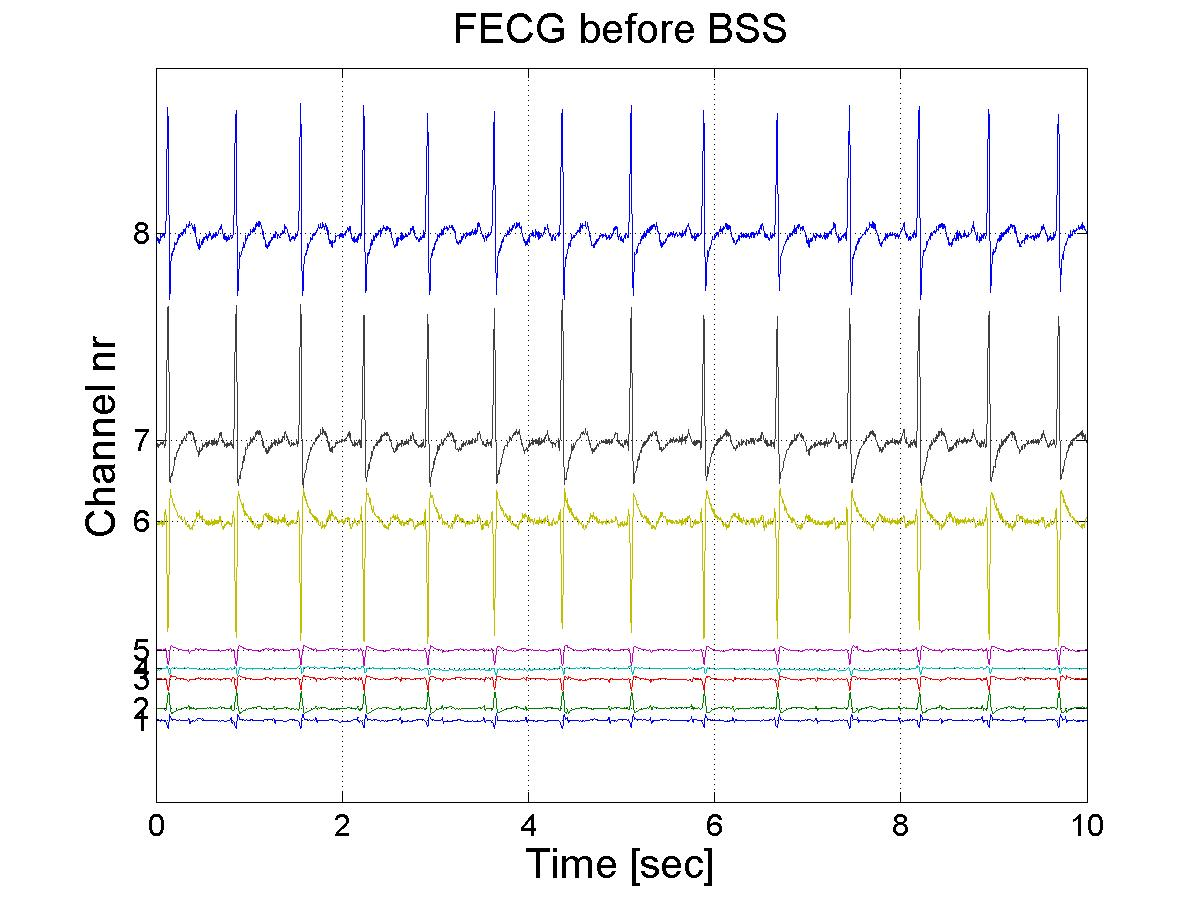
\includegraphics[width=1\linewidth]{100.jpg}
\subcaption{FECG before BSS}\label{FECG2}
\endminipage\hfill
\minipage{0.5\textwidth}%
\centering
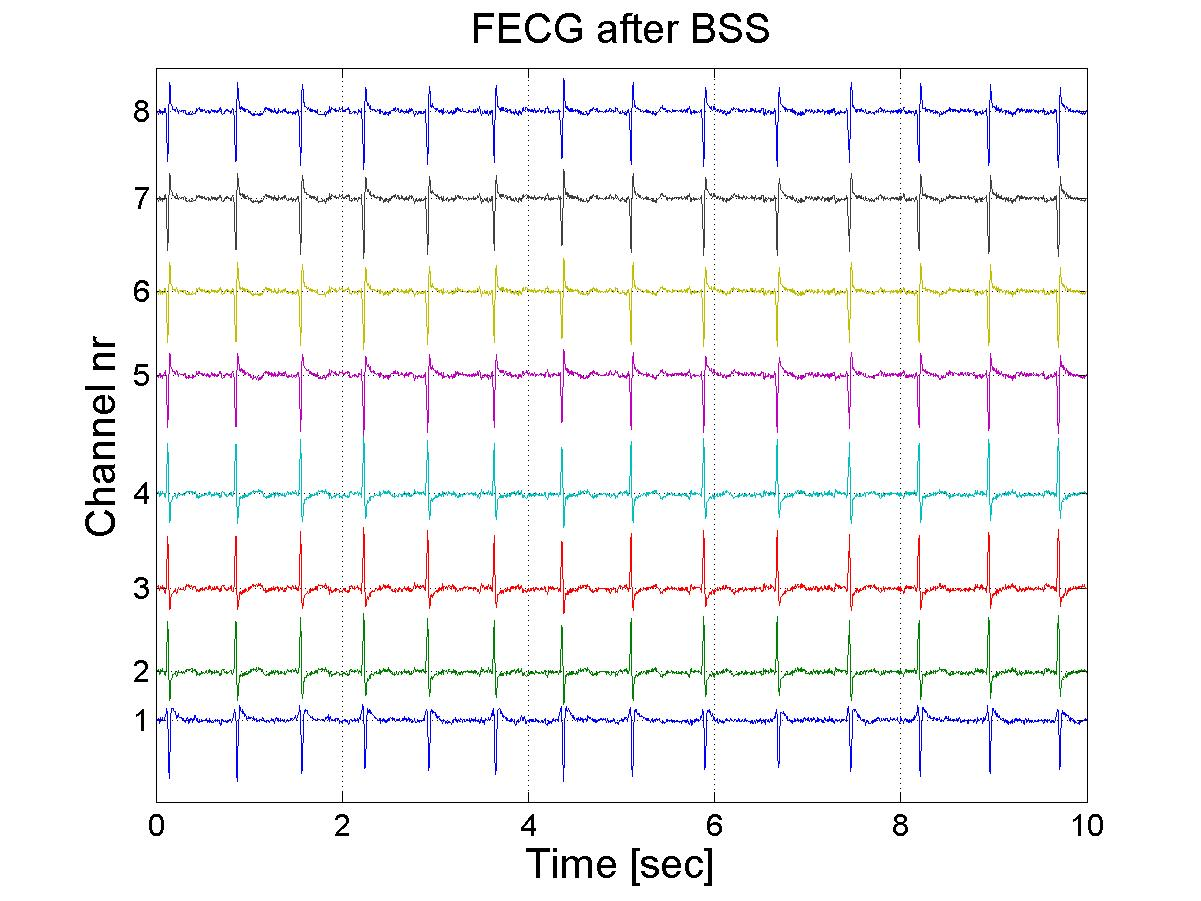
\includegraphics[width=1\linewidth]{101.jpg}
\subcaption{FECG after BSS}\label{FECG1}
\endminipage\hfill
\caption{BSS over FECG.}
\end{figure}
\section{Multi-channel data}

In this study an ultrasound (US) dataset channel data acquired from \href{www.medicalimagingcenter.be/}{MIRC} \footnote{Medical Imaging Research Center UZ Leuven} has been utilized. The goal is to remove the US artefact and filter out the undesired part of the signal. US probe a part from the noisy contaminated signal introduces some DC level as well as low frequency signal at the onset of the time course. This appear in the US image as noise and limit the usability of this method in the near field. Additionally \textbf{\textit{wgn}} is also superimposed in the signal which needs to be removed. The US probe being used has a bandwidth from 2-7 MHz meaning that anything appearing outside this bad is considered to be noise or artefact. In this application EDS is the underlying model to be employed for subspace signal processing. Since the artefact component appear at lower frequencies with significantly higher level compare to the component sitting at the desired bad (DB) (2-7 MHz) figure \ref{US1} it is critically important to remove this component without affecting the rest of the signal. This approach would enable a much better noise suppression. 

Hereby the subspace framework is utilized wherein 28 component are computed. Then the component where their respective frequency sits outside the DB will be deduced from the original signal. The outcome from this is quite on an acceptable range, since the component of the DB sits at high values compare to the rest of the components \ref{US2}. The original and the artefact removed signal in time domain are plotted in figure \ref{UST1} and \ref{UST2} respectively.


\begin{figure}[!htbp]
\minipage{0.5\textwidth}%
\centering
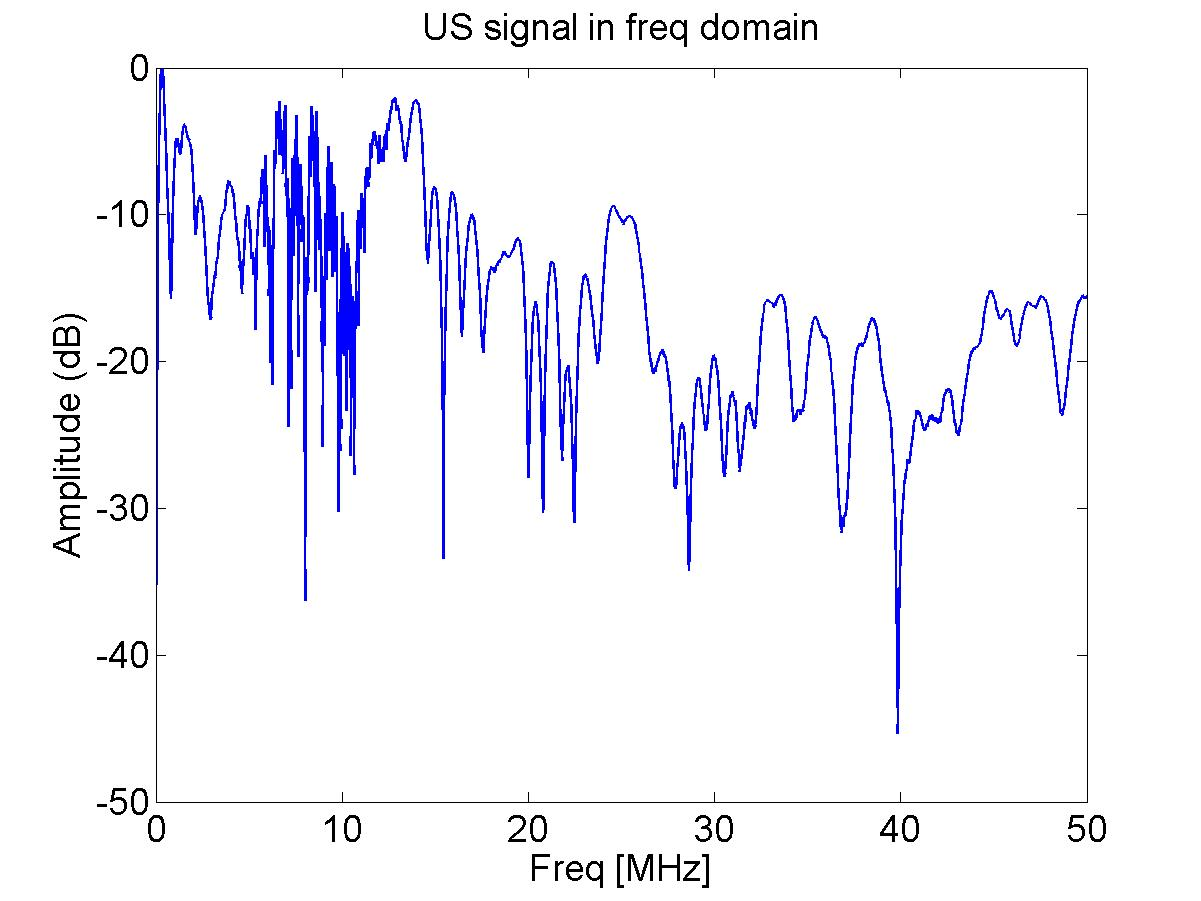
\includegraphics[width=1\textwidth]{800.jpg}
\subcaption{Original signal}\label{US1}
\endminipage\hfill
\minipage{0.5\textwidth}%
\centering
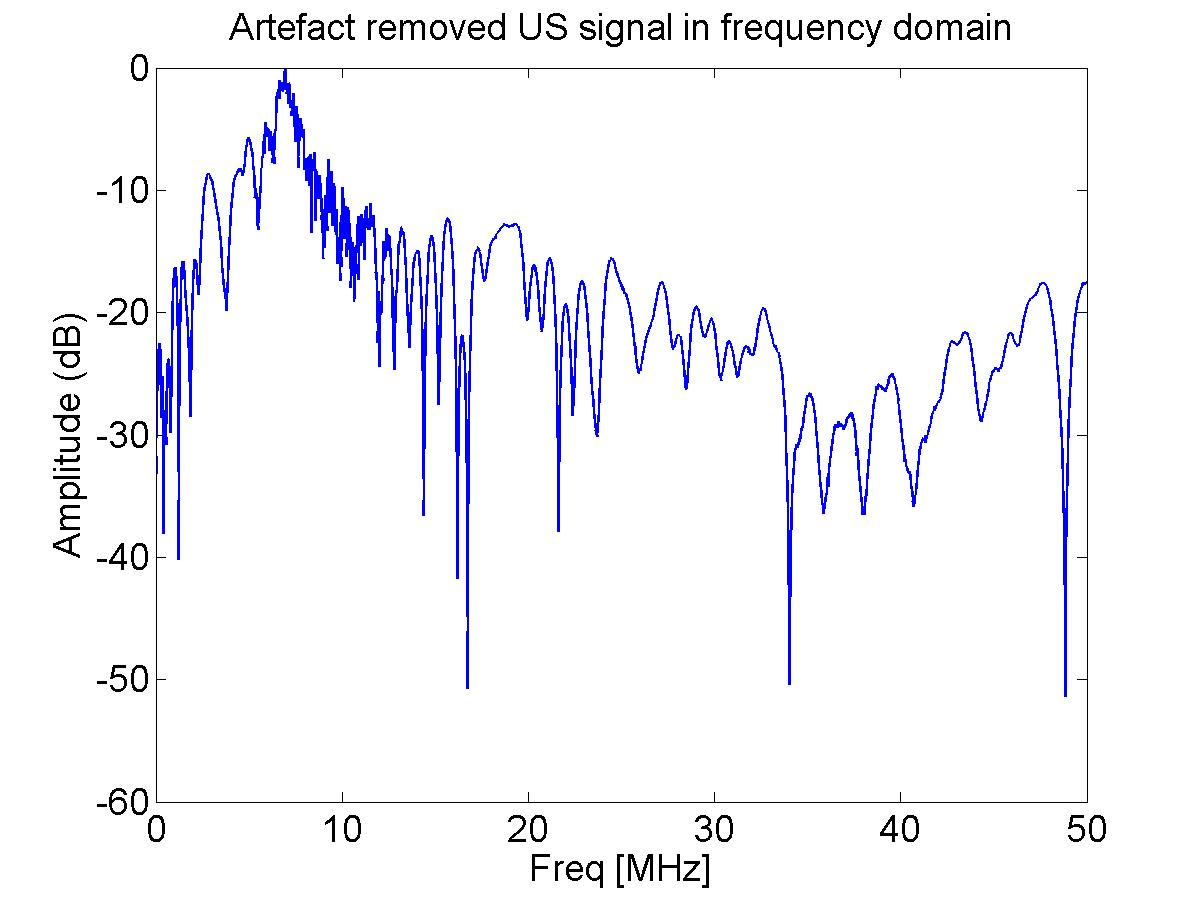
\includegraphics[width=1\textwidth]{801.jpg}
\subcaption{Artefact removed signal}\label{US2}
\endminipage\hfill
\caption{US signals.}
\end{figure}

After completing the artefact removal, signal has to be filtered out via subspace signal processing methods. Single channel algorithm Cadzow and minimum variance are alternative solution however their performance would not be the same as compare to the multichannel version of Cadzow. Single channel would not get into account the common dynamics of the of neighbouring region of interest being scanned as well as the cross talk between neighbouring ultrasound transducers inside the probe. The only drawback associated with multichannel is its time complexity increases significantly as the number of data-points is much higher. Nevertheless this could be a powerful approach for imaging stationary data via echo whereby an increase in image resolution could be achieved. 
 




\begin{figure}[!htbp]
\centering
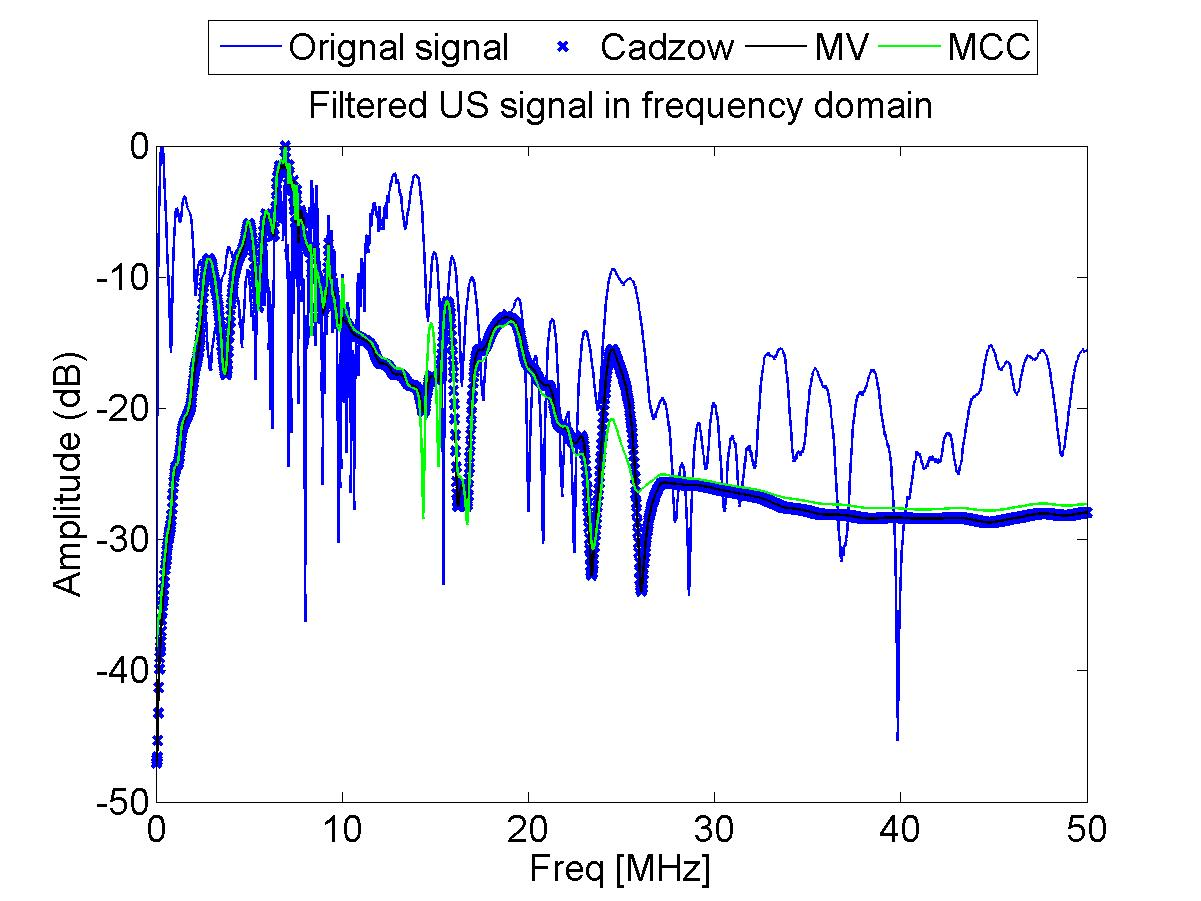
\includegraphics[width=1\textwidth]{802.jpg}
\caption{US filtered signal}\label{US3}
\end{figure}


Since subspace signal processing is a parametric method, component number of the decomposition is the only input required for this underlying model. In this case, 28 components are chosen to be sufficient number since a higher value would not yield significantly better outcome, given the time complexity would increases dramatically. 

Multichannel version would thereby overcome both this obstacles and the outperform both Cadzow and minimum variance. The filtered signal in frequency domain are overlapped in figure \ref{US3} where their respective time domain time course could be found in figure \ref{UST3},\ref{UST4},\ref{UST5}.In figure \ref{US3} are the normalised spectrum where at first glance the the filtering method suppresses the undesired spectrum down to -20 dB whereby the DB is totally untouched. 

\begin{table}[!htbp]
\centering
\caption{SNR evaluation for different methods}\label{tab12}
\begin{tabular}{c c c c c c} 
\hline 
$ $&$Original Signal$&$Cadzow$&$MV$&$MCC$ \\\hline 
            
$SNR$&$ -5.2161 $&$ 10.3109 $&$ 10.3109  $&$ 10.7620$\\
\hline 
\end{tabular}
\end{table}

In order to testify the performance of these filtering method the SNR has been computed via equation \ref{SNR1} in the frequency domain. The numerator is the variance of the DB whereas the denominator is the variance of all the components outside the DB. In table \ref{tab12} are the SNR listed where it could be increase of signal quality where the multichannel case outperforms the rest of the methods. Quite important to mention that high dynamics of the signal (very high frequency components) being filtered out via multichannel is visually notable in figure \ref{US3}.


\section{Epilepsy data}


\begin{figure}[!htbp]
\minipage{0.5\textwidth}%
\centering
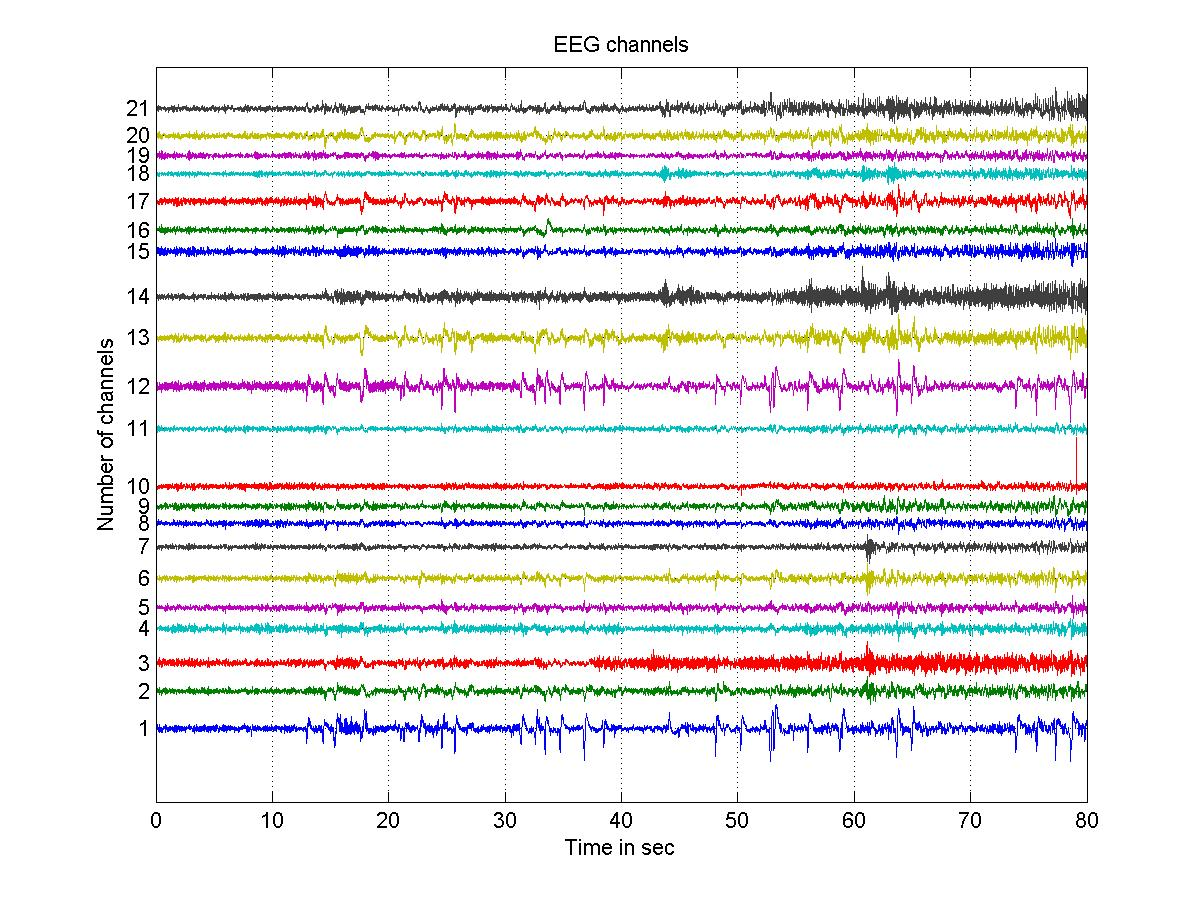
\includegraphics[width=1\linewidth]{300.jpg}
\subcaption{EEG signal}
\endminipage\hfill
\minipage{0.5\textwidth}%
\centering
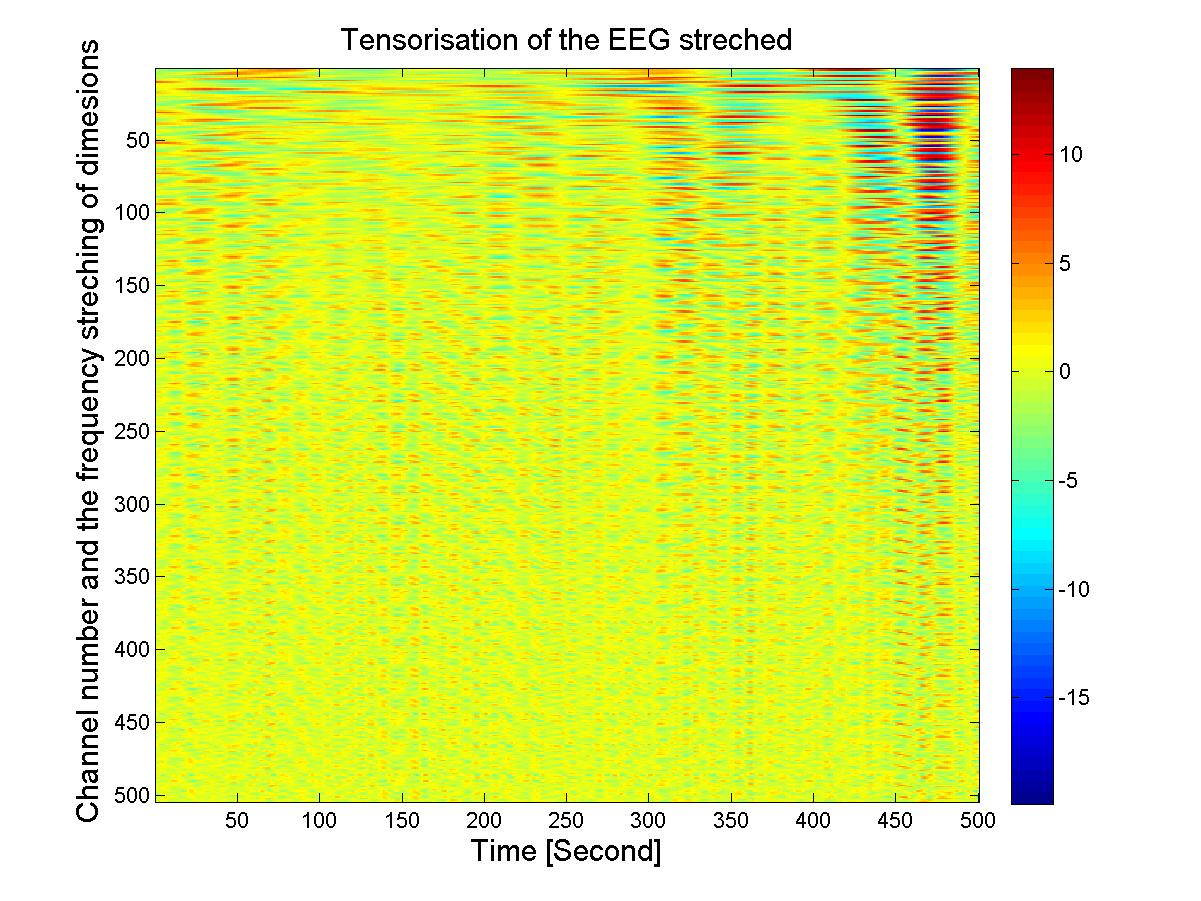
\includegraphics[width=1\linewidth]{301.jpg}
\subcaption{Unfolded Tensor.}
\endminipage\hfill
\caption{EEG signal and its tensor of 21*24*500 dimensions unfolded into  504x500 matrix}
\end{figure}

The EEG data set is structured into different channel data over a time course of 80 sec. An epileptic seizure has been detected at around t=52 sec. In order to map this signal into a head model, BSS has to be performed over the dataset. Hereby the normal brain activity has to be separated from the epilepsy. Tensorisation has to be formed via wavelet transform. The outcome will be a third order tensor where its respective orders are time, frequency and the number of channels. 

In order to estimate the rank of this tensor, the performance of CPD has been tested over different rank trials. In figure \ref{CPD-4} the plots clearly testify the fastest convergence for a rank two computation. 

\begin{figure}[!htbp]
\centering
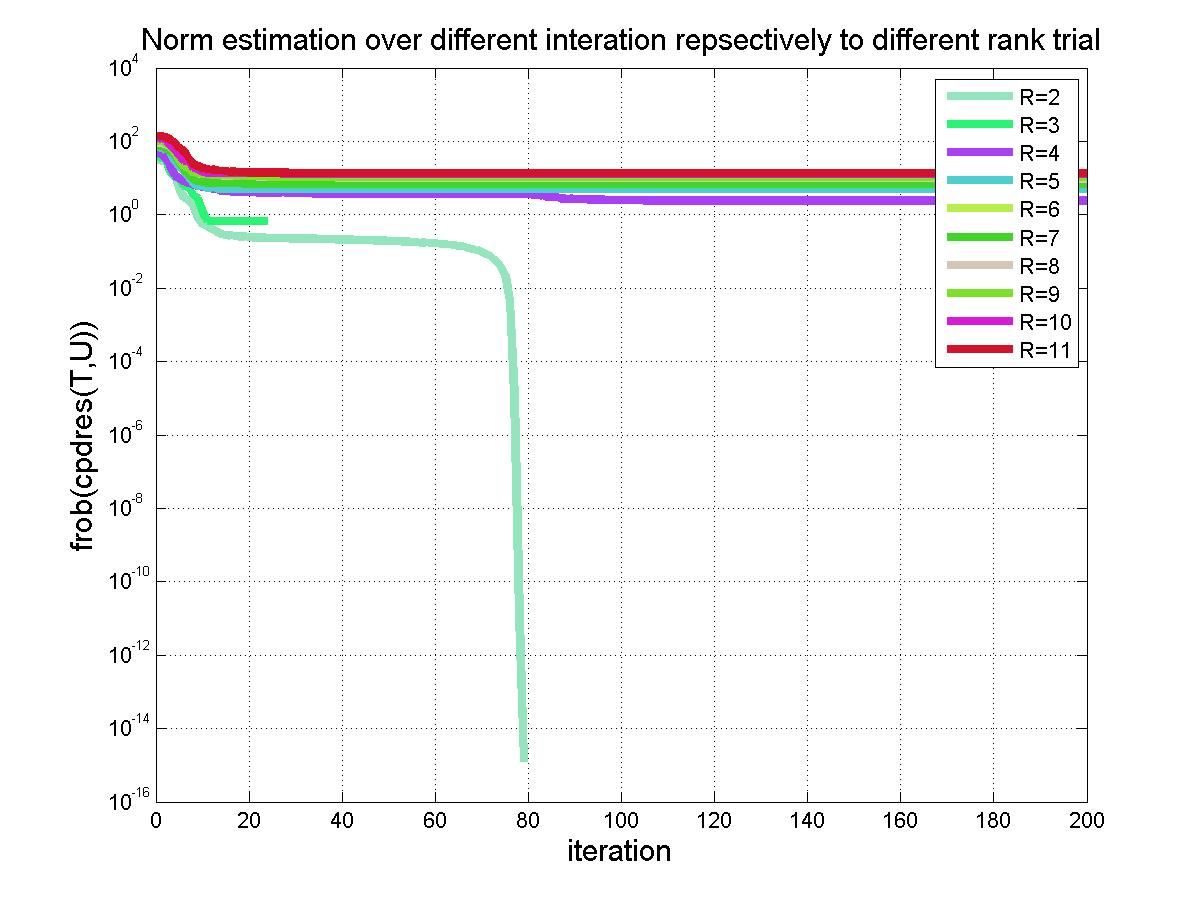
\includegraphics[width=0.5\linewidth]{304.jpg}
\caption{CPD performance}\label{CPD-4}
\end{figure}


Therefore the number of rank one tensor correspond to distinct uncorrelated event encoded into the EEG signals. Epilepsy as the first component together with the normal brain activity signals are both superimposed. Since CPD ensures a unique BSS the event are efficiently separated and their potential distribution into a spherical head model produces completely different potential map. 

Epilepsy is mostly associated with high frequency variations in the EEG signals whereas a brain activity stands mostly a low frequencies. 

In order to testify this the first mode of the decomposition has been plotted in figure \ref{AC1} and \ref{AC2}. The frequency component in figure \ref{AC1} for the highest variation in frequency is quite irregular and chaotic behaviour. This has been associated to epilepsy. This is also the case in higher order component of the temporal signature in figure \ref{AC2} where a more pronounced chaotic behaviour is outlined for the seizure.



\begin{figure}[!htbp]
\minipage{0.5\textwidth}%
\centering
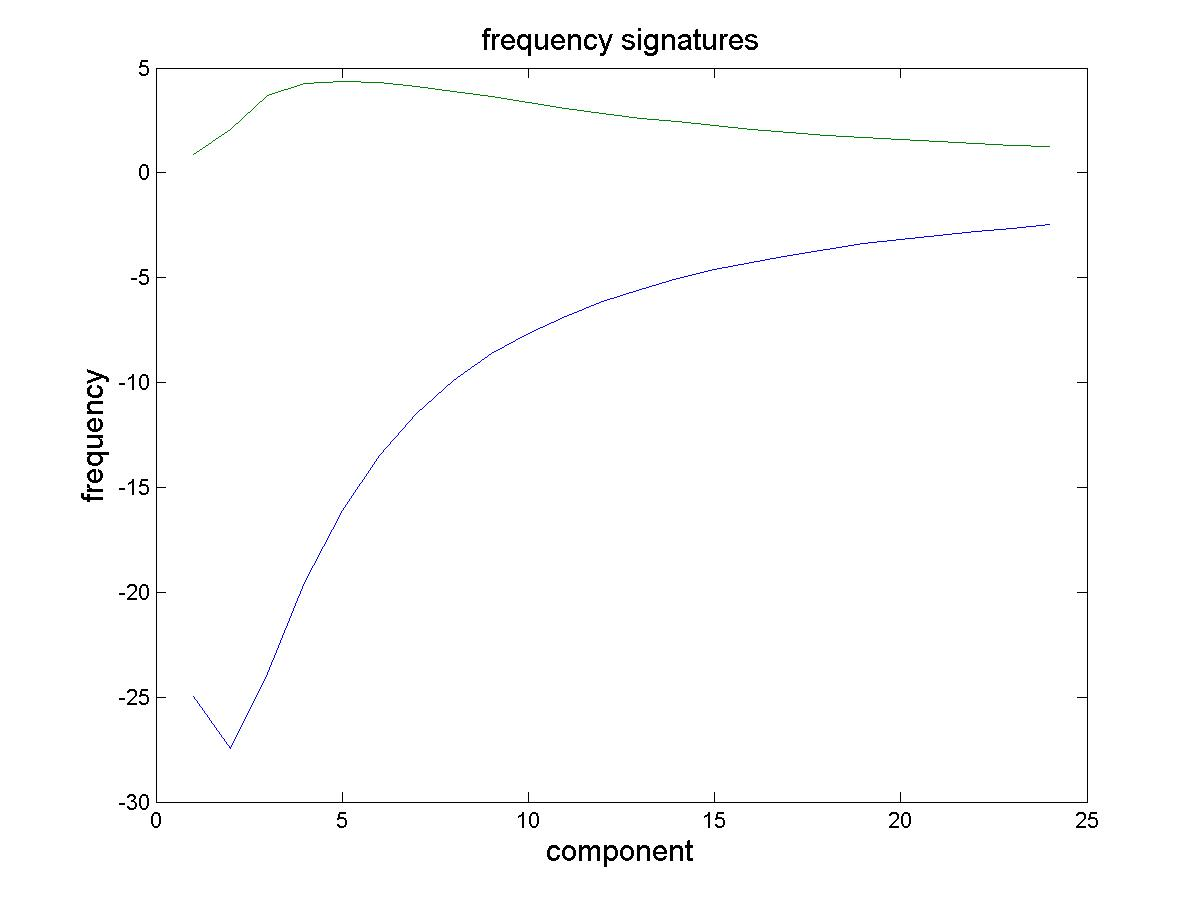
\includegraphics[width=1\linewidth]{302.jpg}
\subcaption{Frequency components}\label{AC1}
\endminipage\hfill
\minipage{0.5\textwidth}%
\centering
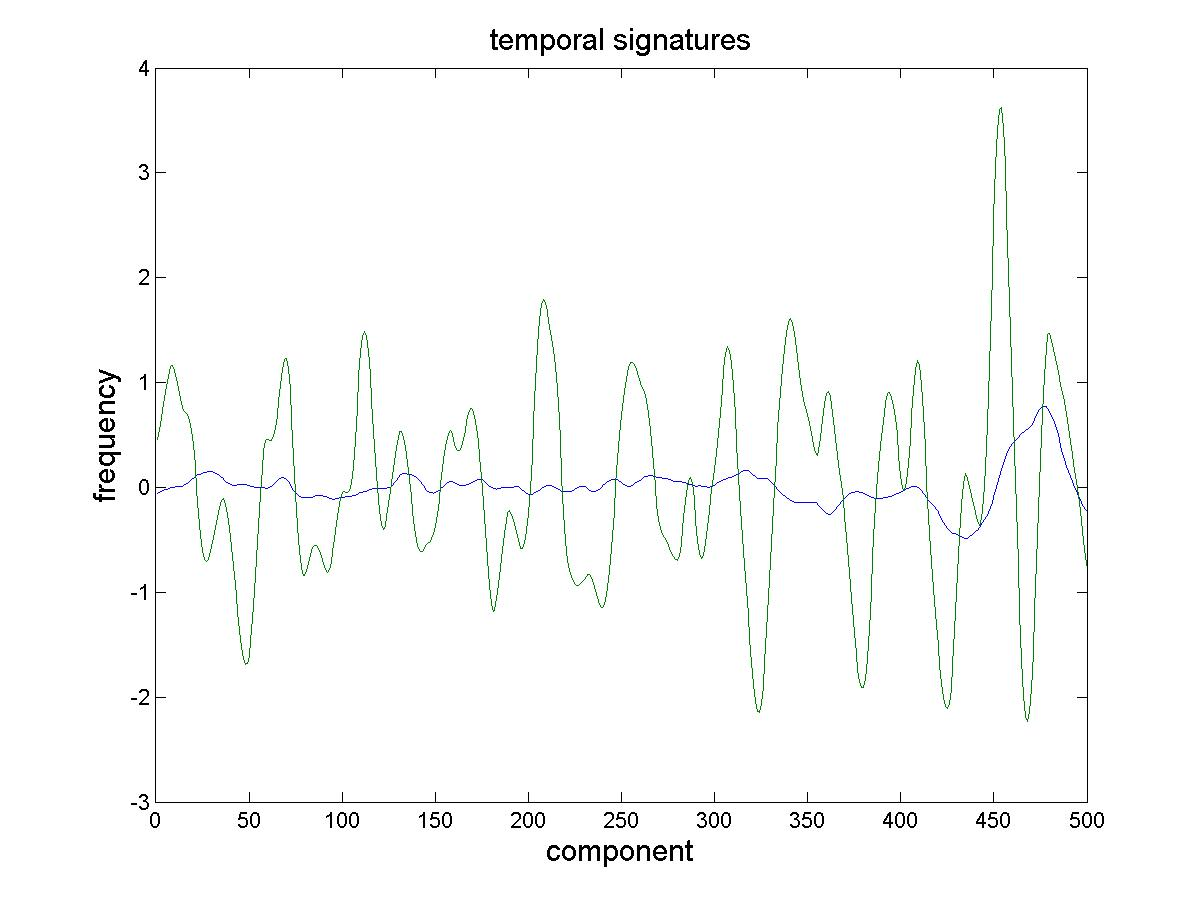
\includegraphics[width=1\linewidth]{303.jpg}
\subcaption{Time course activity}\label{AC2}
\endminipage\hfill
\caption{Plots of distinct events}
\end{figure}

These two event are mapped into a spherical head model in figure \ref{AC3} is the seizure located on top of the head whereas the second component which is the normal brain activity is potential distribution in figure \ref{AC4}.


\begin{figure}[!htbp]
\minipage{0.5\textwidth}%
\centering
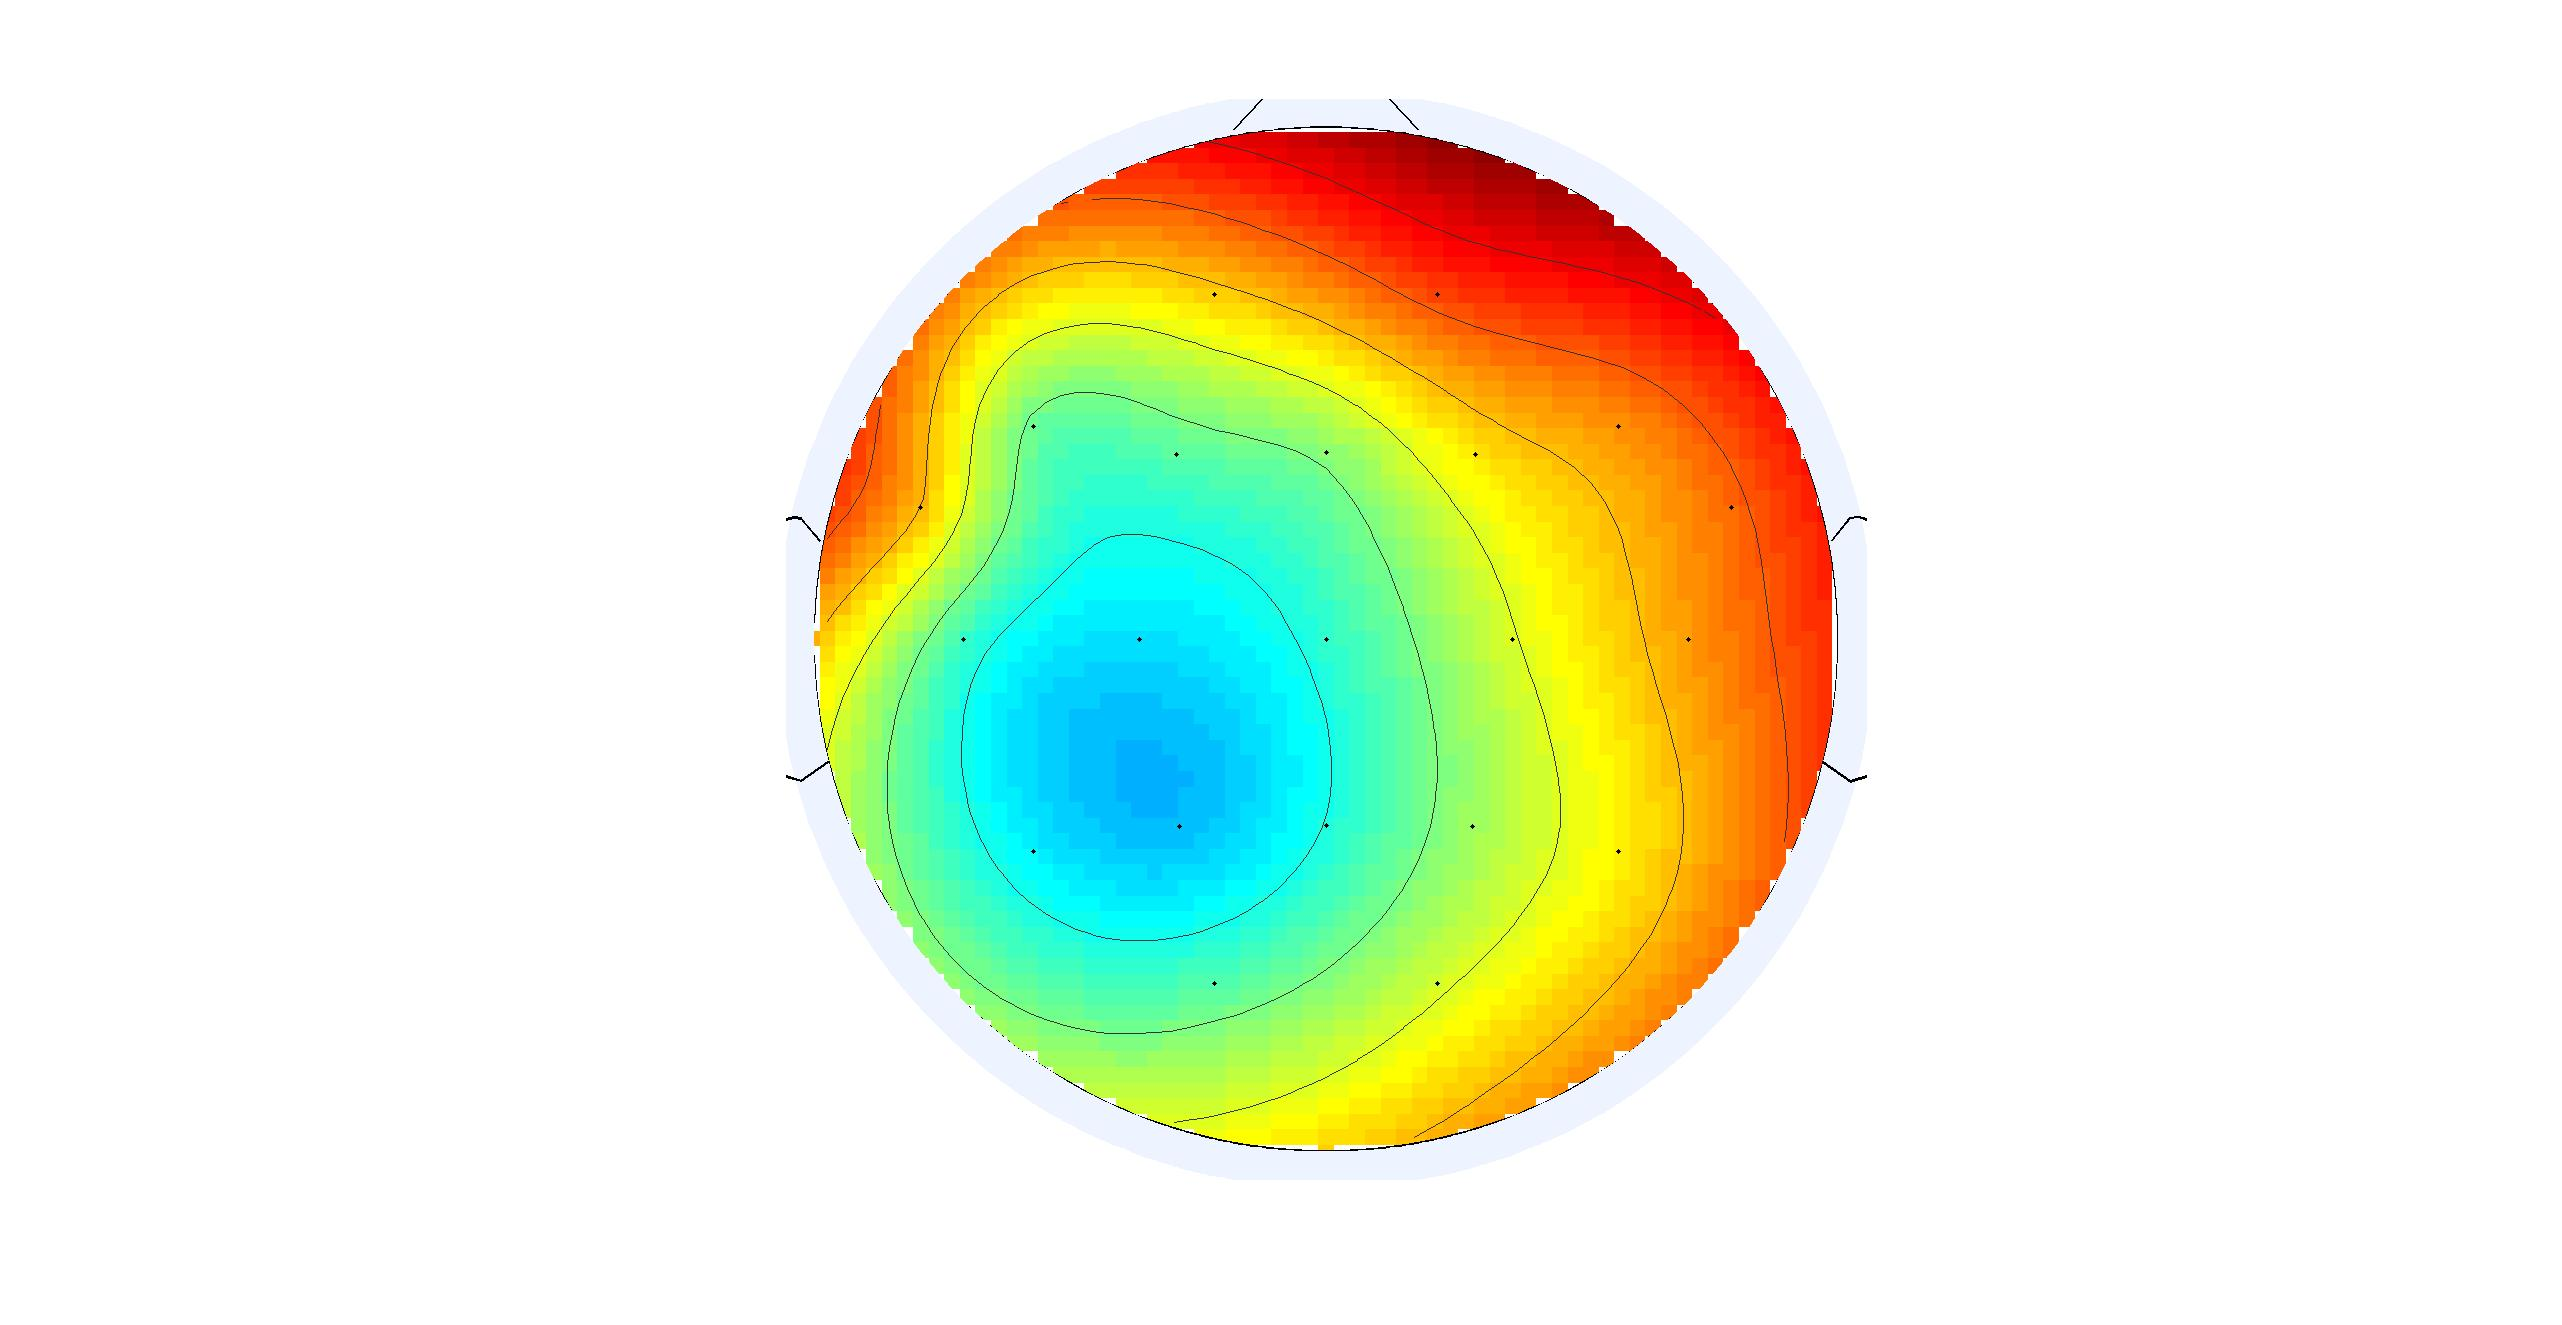
\includegraphics[width=1\linewidth]{305.jpg}
\subcaption{Seizure.}\label{AC3}
\endminipage\hfill
\minipage{0.5\textwidth}%
\centering
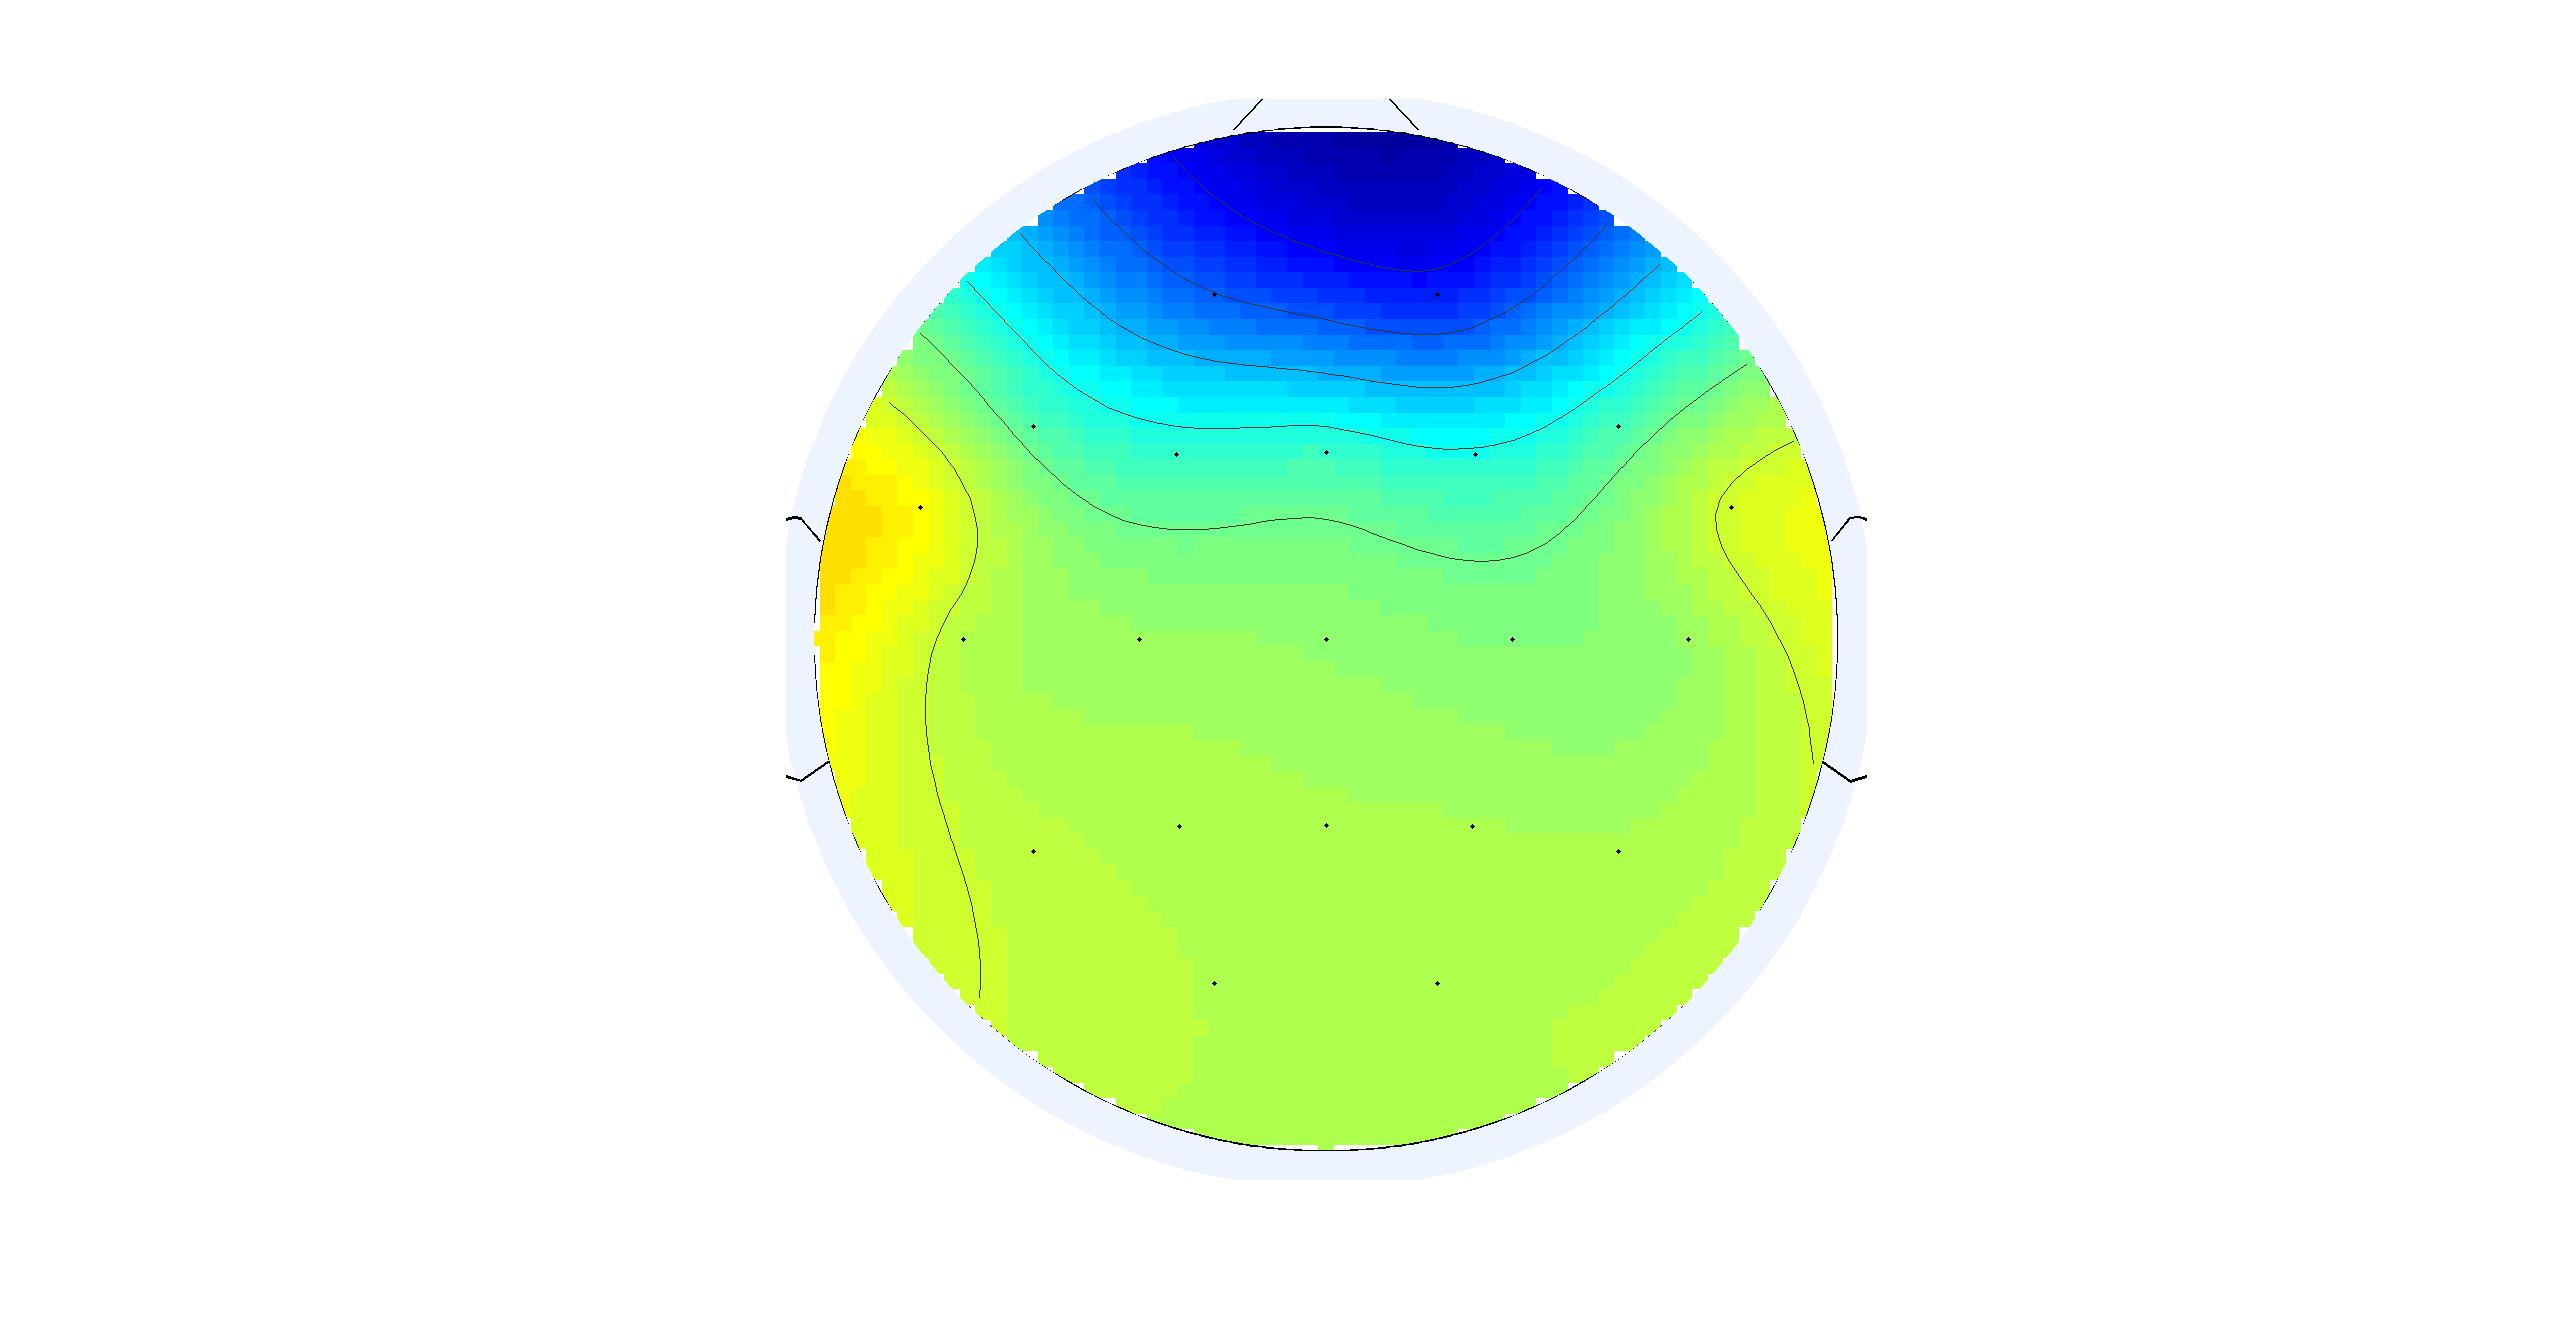
\includegraphics[width=1\linewidth]{307.jpg}
\subcaption{Normal activity}\label{AC4}
\endminipage\hfill
\caption{Potential distribution of these two events}
\end{figure}


\clearpage
\bibliographystyle{unsrt}
\bibliography{Bibliography3}


\clearpage
\appendix

\section{Appendix}

\subsection{Testing Fast-ICA}\label{A1}

\begin{figure}[!htbp]
\minipage{0.5\textwidth}%
\centering
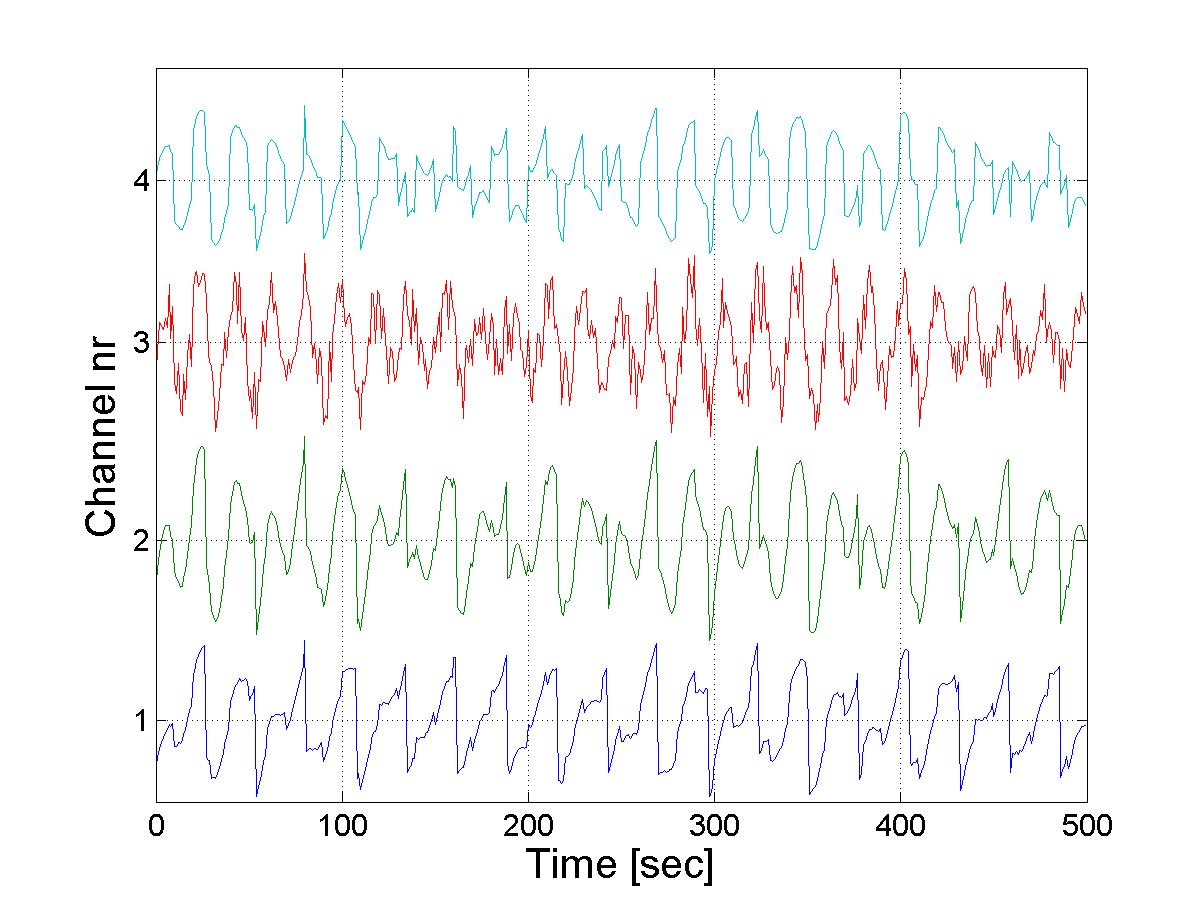
\includegraphics[width=1\linewidth]{13.jpg}
\subcaption{Before ICA}
\endminipage\hfill
\minipage{0.5\textwidth}%
\centering
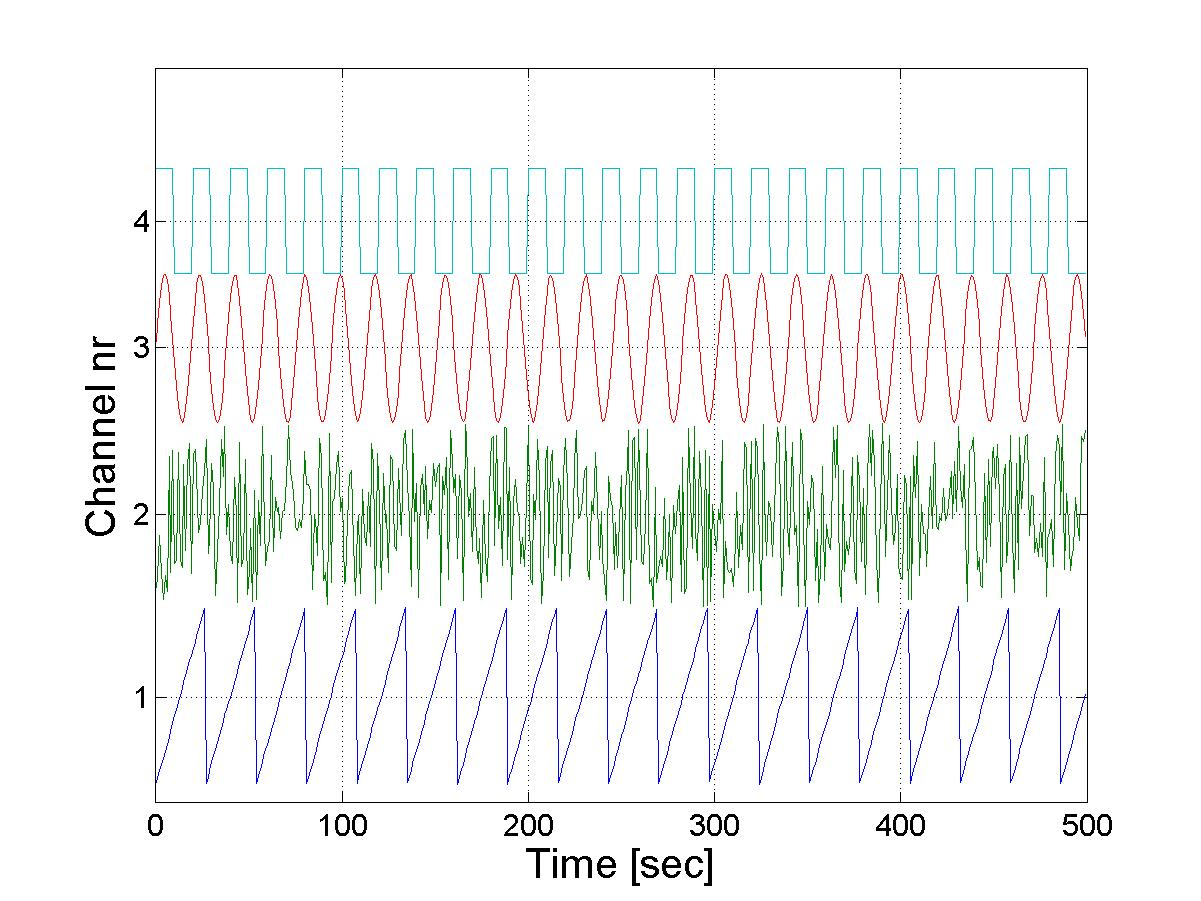
\includegraphics[width=1\linewidth]{14.jpg}
\subcaption{After ICA}
\endminipage\hfill
\caption{Test ICA}
\end{figure}

\subsection{Mixing matrix}\label{A2}

\begin{equation}
A_{1}=\frac{1}{\sqrt{5}}    
\bigg\{
 \begin{matrix}
  1 & -2 \\
  -2 & 1 
 \end{matrix}
\bigg\}
\end{equation}

\begin{equation}
A_{2}=\frac{1}{\sqrt{2.21}}    
\bigg\{
 \begin{matrix}
  1 & -1.1 \\
  -1.1 & 1 
 \end{matrix}
\bigg\}
\end{equation}
\section{HRV appendix}
\subsection{\small ECG signal processing}


\begin{figure}[!htbp]
    \centering
    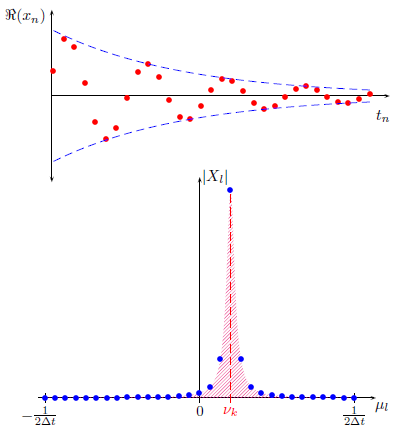
\includegraphics[width=0.5\textwidth]{icon3.png}
    \caption{Electrod placement}
    \label{icon3}
\end{figure}

\begin{figure}[!htbp]
\minipage{0.5\textwidth}%
\centering
    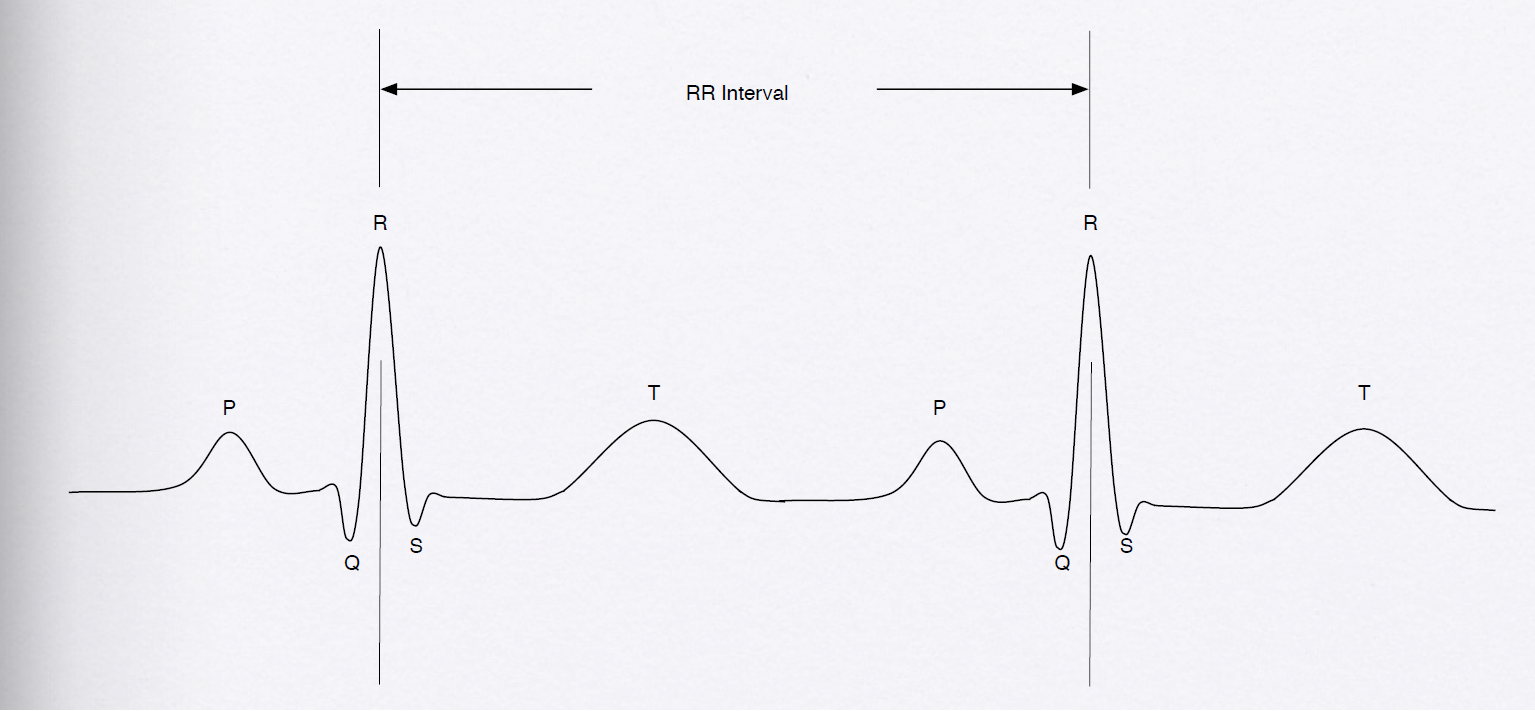
\includegraphics[width=1\textwidth]{icon4.png}
    \subcaption{Outline of heartbeat signal}
\endminipage\hfill
\minipage{0.5\textwidth}%
\centering
    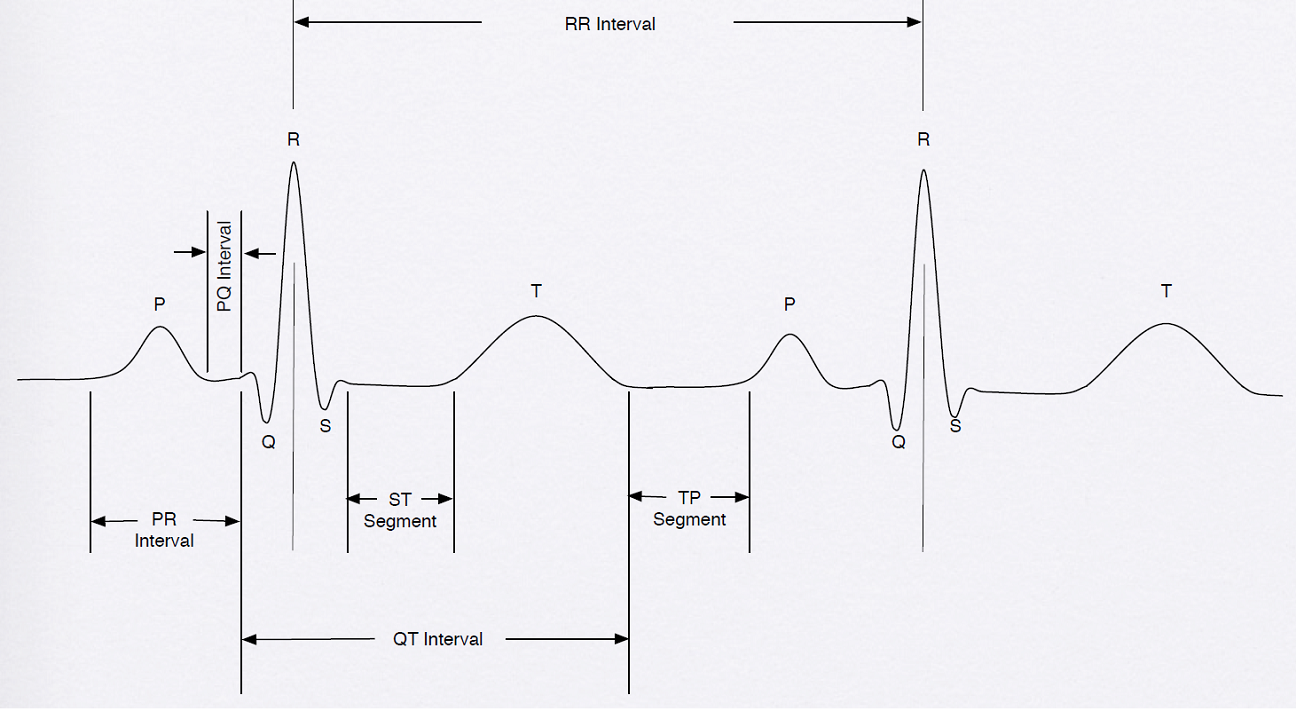
\includegraphics[width=0.9\textwidth]{icon5.png}
    \subcaption{Detailed segmentation of the signal}
\endminipage\hfill
\caption{QRS signal time course}\label{icon4}
\end{figure}

\begin{figure}[!htbp]
\minipage{0.5\textwidth}%
\centering
\begin{itemize}
    \item P wave: depolarisation of atria
    \item QRS complex: depolarisation of ventricles
\end{itemize}
\endminipage\hfill
\minipage{0.5\textwidth}%
\centering
\begin{itemize}
    \item T wave: ventricle re-polarisation
    \item U wave: atria re-polarisation
\end{itemize}
\endminipage\hfill
\caption{QRS signal time course}\label{icon4}
\end{figure}



\newpage
\subsection{\small Pan-Tomkins}\label{algo1}

\begin{figure}[!htbp]
\centering
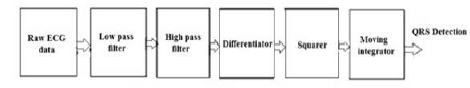
\includegraphics[width=0.6\linewidth]{pan_tomkins.png}
\caption{Pan Tomkins}
\end{figure}


\newpage
\subsection{\small RR time course for each subject of respective group}\label{RR}

\begin{figure}[!htbp]
\foreach \i in {121,...,130} {%
    \begin{subfigure}[p]{0.5\textwidth}
        \includegraphics[width=0.6\linewidth]{\i}
    \end{subfigure}\quad
}
\end{figure}


\newpage
\subsection{\small Pointcare plots}\label{PC}

\begin{figure}[!htbp]
\foreach \i in {131,...,140} {%
    \begin{subfigure}[p]{0.5\textwidth}
        \includegraphics[width=0.6\linewidth]{\i}
    \end{subfigure}\quad
}
\end{figure}

\newpage
\subsection{\small ACF plots}\label{ACF}

\begin{figure}[!htbp]
\foreach \i in {141,...,150} {%
    \begin{subfigure}[p]{0.5\textwidth}
        \includegraphics[width=0.6\linewidth]{\i}
    \end{subfigure}\quad
}
\end{figure}

\newpage
\subsection{\small Phase space plots}\label{PSP}

\begin{figure}[!htbp]
\foreach \i in {151,...,160} {%
    \begin{subfigure}[p]{0.5\textwidth}
        \includegraphics[width=0.6\linewidth]{\i}
    \end{subfigure}\quad
}
\end{figure}

\newpage
\subsection{\small f-slope plots}

\begin{figure}[!htbp]
\foreach \i in {161,...,170} {%
    \begin{subfigure}[p]{0.5\textwidth}
        \includegraphics[width=0.6\linewidth]{\i}
    \end{subfigure}\quad
}
\end{figure}

\newpage
\subsection{\small Hurst exponential plots}

\begin{figure}[!htbp]
\foreach \i in {171,...,180} {%
    \begin{subfigure}[p]{0.5\textwidth}
        \includegraphics[width=0.6\linewidth]{\i}
    \end{subfigure}\quad
}
\end{figure}

\newpage
\subsection{\small Box counting plots}

\begin{figure}[!htbp]
\foreach \i in {181,...,190} {%
    \begin{subfigure}[p]{0.5\textwidth}
        \includegraphics[width=0.6\linewidth]{\i}
    \end{subfigure}\quad
}
\end{figure}




\newpage
\subsection{\small DFA plots}\label{DFAplots}

\begin{figure}[!htbp]
\foreach \i in {191,...,194} {%
    \begin{subfigure}[p]{0.5\textwidth}
        \includegraphics[width=0.6\linewidth]{\i}
    \end{subfigure}\quad
}
\end{figure}

\newpage
\subsection{\small Cumulative plots}\label{CP}

\begin{figure}[!htbp]
\foreach \i in {195,...,204} {%
    \begin{subfigure}[p]{0.5\textwidth}
        \includegraphics[width=0.6\linewidth]{\i}
    \end{subfigure}\quad
}
\end{figure}



\newpage
\subsection{\small Control dataset Correlation dimension plots}

\begin{figure}[!htbp]
\foreach \i in {205,...,214} {%
    \begin{subfigure}[p]{0.5\textwidth}
        \includegraphics[width=0.6\linewidth]{\i}
    \end{subfigure}\quad
}
\end{figure}

\newpage
\subsection{\small Control dataset Correlation dimension plots}
\begin{figure}[!htbp]
\foreach \i in {215,...,224} {%
    \begin{subfigure}[p]{0.5\textwidth}
        \includegraphics[width=0.6\linewidth]{\i}
    \end{subfigure}\quad
}
\end{figure}


\newpage
\subsection{\small Linear regression for window size 16 samples.}\label{LR}

\begin{figure}[!htbp]
\foreach \i in {225,...,234} {
    \begin{subfigure}[p]{0.5\textwidth}
        \includegraphics[width=0.6\linewidth]{\i}
    \end{subfigure}\quad
}
\end{figure}



\end{figure}


\lstset{language=Matlab,%
    %basicstyle=\color{red},
    breaklines=true,%
    morekeywords={matlab2tikz},
    keywordstyle=\color{blue},%
    morekeywords=[2]{1}, keywordstyle=[2]{\color{black}},
    identifierstyle=\color{black},%
    stringstyle=\color{mylilas},
    commentstyle=\color{mygreen},%
    showstringspaces=false,%without this there will be a symbol in the places where there is a space
    numbers=left,%
    numberstyle={\tiny \color{black}},% size of the numbers
    numbersep=9pt, % this defines how far the numbers are from the text
    emph=[1]{for,end,break},emphstyle=[1]\color{red}, %some words to emphasise
    %emph=[2]{word1,word2}, emphstyle=[2]{style},   
    backgroundcolor=\color{backcolour},   
    commentstyle=\color{codegreen},
    %keywordstyle=\color{magenta},
    numberstyle=\tiny\color{codegray},
    stringstyle=\color{codepurple},
    basicstyle=\footnotesize,
    breakatwhitespace=false,         
    breaklines=true,                 
    captionpos=b,                    
    keepspaces=true,                 
    numbers=left,                    
    numbersep=5pt,                  
    showspaces=false,                
    showstringspaces=false,
    showtabs=false,                  
    tabsize=2
}

\newpage
\section{Main code}

\subsection{Part 1}
\lstinputlisting{Main_Session_Part_1.m}
\subsection{Part 2}
\lstinputlisting{Main_Session_Part_2.m}
\subsection{Part 3}
\lstinputlisting{Main_Session_Part_3.m}
\subsection{Part 4}
\lstinputlisting{Main_Session_Part_4.m}
\subsection{Aid functions}
\lstinputlisting{Vangjus_Part_Per_Million2_k_Hz.m}
\lstinputlisting{Vangjush_Antidiag.m}
\lstinputlisting{Vangjush_Avg_Hankel_Matrix.m}
\lstinputlisting{Vangjush_Correct_Signular.m}
\lstinputlisting{Vangjush_Cadzow.m}
\lstinputlisting{Vangjush_Costum.m}
\lstinputlisting{Vangjush_Costum_Plot.m}
\lstinputlisting{Vangjush_Costum_Plot1.m}
\lstinputlisting{Vangjush_Extract_Signal.m}
\lstinputlisting{Vangjush_ExtractionNeigbours.m}
\lstinputlisting{Vangjush_Filter_MRS_Signal.m}
\lstinputlisting{Vangjush_Filter_Water_Signal.m}
\lstinputlisting{Vangjush_Freq_Damping_Esti.m}
\lstinputlisting{Vangjush_Hankel_Matrix.m}
\lstinputlisting{Vangjush_Header_2_Latex_Table.m}
%\lstinputlisting{Vangjush_Header_2_Latex_Table1.m}
\lstinputlisting{Vangjush_Parameter_2_Latex_Table.m}
\lstinputlisting{Vangjush_HSVD.m}
\lstinputlisting{Vangjush_HTLSU.m}
\lstinputlisting{Vangjush_HTLSU_PK_FD.m}
\lstinputlisting{Vangjush_Linear_Parameter_Estination.m}
\lstinputlisting{Vangjush_MDL.m}
\lstinputlisting{Vangjush_Mean_Variance_2_Latex_Table.m}
\lstinputlisting{Vangjush_Multi_Channel_Cadzow.m}
\lstinputlisting{Vangjush_Multi_Channel_Enhanced.m}
\lstinputlisting{Vangjush_Parameter_2_Latex_Table.m}
\lstinputlisting{Vangjush_Phase_Correction.m}
\lstinputlisting{Vangjush_Phase_Estimation.m}
\lstinputlisting{Vangjush_Plot_Individual_Component.m}
\lstinputlisting{Vangjush_PPM_Axis_Find.m}
\lstinputlisting{Vangjush_Reconstruct_Components.m}
\lstinputlisting{Vangjush_RMSE.m}
\lstinputlisting{Vangjush_RMSE_PartII.m}
\lstinputlisting{Vangjush_Save_Images.m}
\lstinputlisting{Vangjush_TLS.m}
\lstinputlisting{Vangjush_Truncate_SVD.m}
\lstinputlisting{Vangjush_Vandermond_Tq_Matrix.m}
\lstinputlisting{Vangjush_Walk_Edit_Antidiagonal.m}
\lstinputlisting{Vangush_Minimum_Variance.m}
\lstinputlisting{Vanngjush_Signal_Display.m}










\end{document}

